 %%
%% This is file `kth-ex1.tex',
%% generated with the docstrip utility.
%%
%% The original source files were:
%%
%% kthesis.dtx  (with options: `ex1')
%% 
%% IMPORTANT NOTICE:
%% 
%% For the copyright see the source file.
%% 
%% Any modified versions of this file must be renamed
%% with new filenames distinct from kth-ex1.tex.
%% 
%% For distribution of the original source see the terms
%% for copying and modification in the file kthesis.dtx.
%% 
%% This generated file may be distributed as long as the
%% original source files, as listed above, are part of the
%% same distribution. (The sources need not necessarily be
%% in the same archive or directory.)
\documentclass[ebook,11pt,exjobb]{kth-mag}
\usepackage[T1]{fontenc}
\usepackage{textcomp}
\usepackage{lmodern}
\usepackage[utf8]{inputenc}
\usepackage[english,swedish]{babel}
\usepackage{modifications}
\usepackage{csquotes}
\usepackage{float}
\usepackage{csquotes}
\usepackage[export]{adjustbox}
\usepackage{acronym}
\usepackage{hyperref}
\usepackage{tikz}
\usepackage{float}
\usepackage{pgffor}
\usetikzlibrary{shadows}
\usepackage{xcolor}
\usepackage{amsmath}
\usepackage{amssymb}
\usepackage{relsize}%
\usepackage[final]{pdfpages}
\usepackage{multicol}
\usepackage{pgfplots}
\pgfplotsset{compat=newest}
\usepackage{enumitem}
\usepackage{tabularx,booktabs}
\usetikzlibrary{matrix,chains,positioning,decorations.pathreplacing,arrows,shapes.gates.logic.US,shapes.gates.logic.IEC,calc,3d,shapes.geometric}
\usepackage[
backend=biber,
style=ieee,
citestyle=ieee 
]{biblatex}

\usepackage{rotating}
\usepackage{makecell, multirow}
\renewcommand\theadfont{\normalsize}
\renewcommand\theadgape{}

\newcolumntype{C}{>{\centering\arraybackslash}X} % centered version of "X" type
\setlength{\extrarowheight}{1pt}

\pgfmathdeclarerandomlist{MyRandomColors}{%
    {white}%
    {white}%    
    {white}%
    {white}%
    {white}%
    {white}%
    {white}%
    {white}%
    {black}%
    {white}%
    {white}%
    {white}%
    {white}%
    {black}%
    {white}%
    {white}%
    {white}%
}%

\newcommand*{\GridSize}{35}

\newcommand*{\ColorCells}{%
    \foreach \y in {1,...,\GridSize} {
        \foreach \x in {1,...,\GridSize} {
            \pgfmathrandomitem{\RandomColor}{MyRandomColors} 
            \draw [fill=\RandomColor, draw=none, ultra thick] 
                (\x-1,\y-1) rectangle (\x,\y);
        }%
    }%
}%

\listfiles

\DeclareMathOperator*{\argmax}{arg\,max}



\title{Using Neurobiological Frameworks for Anomaly Detection in System Log Streams}
\foreigntitle{Anomali Detektion i System Loggar med Hjälp av Neurobiologiskt Ramverk}
\author{Gustaf Rydholm}
\date{2018}
\blurb{\hfill\\\hfill\\\hfill\\\hfill\\\hfill\\\hfill\\Examiner: Joakim Jaldén\\Academic Supervisor: Arun Venkitaraman\\Industrial Supervisor at Ericsson: Armin Catovic\\\hfill\\Master's Thesis in Signal Processing\\School of Electrical Engineering and Computer Science\\Royal Institute of Technology, SE-100 44 Stockholm, Sweden\\Stockholm, Sweden 2018}
\trita{}%TRITA-EE-EX-2018:nn




\addbibresource{references/ref.bib}

\begin{document}


\includepdf[fitpaper=true, pages={1}]{FrontAndBackPage/neurobio.pdf}
\clearpage\thispagestyle{empty}\mbox{}\clearpage
\maketitle
\selectlanguage{english}
\frontmatter
\pagestyle{empty}

%\removepagenumbers

%%
%% This is file `kth-abs.tex',
%% generated with the docstrip utility.
%%
%% The original source files were:
%%
%% kthesis.dtx  (with options: `abstract')
%% 
%% IMPORTANT NOTICE:
%% 
%% For the copyright see the source file.
%% 
%% Any modified versions of this file must be renamed
%% with new filenames distinct from kth-abs.tex.
%% 
%% For distribution of the original source see the terms
%% for copying and modification in the file kthesis.dtx.
%% 
%% This generated file may be distributed as long as the
%% original source files, as listed above, are part of the
%% same distribution. (The sources need not necessarily be
%% in the same archive or directory.)
\begin{abstract}
  \textit{Artificial Intelligence} (AI) has shown enormous potential, and is predicted to be a prosperous field that will likely revolutionise entire industries and bring forth a new industrial era. However, most of today's AI is either, as in deep learning, an oversimplified abstraction of how an actual mammalian brains neural network function, or methods sprung from mathematics. But, with the foundation of the bold ideas of Vernon Mountcastle stated in 1978 about the neocortical functionality, new frameworks for creating true machine intelligence have been developed, and continues to be. 
  
  In this thesis, we study one such theory, called \textit{Hierarchical Temporal Memory} (HTM). We use this framework to build a machine learning model in order to solve the task of detecting and classifying anomalies in system logs belonging to Ericsson's component based architecture applications. The results are then compared to an existing classifier, called \textit{Linnaeus}, which uses classical machine learning methods. The HTM model is able to show promising capabilities of classifying system log sequences with similar results compared with the Linnaeus model. The HTM model is an appealing alternative, due to the limited need of computational resources and the algorithms ability to effectively learn with \textit{``one-shot learning''}.

\end{abstract}
\endinput
%%
%% End of file `kth-abs.tex'.

\clearpage

\begin{foreignabstract}{swedish}
    \textit{Artificiell Intelligens} (AI) har visat enorm potential och är förutspådd att revolutionera hela industrier och introducera en ny industriell era. Men, mestadelen av dagens AI är antingen optimerings algoritmer, eller som med deep learning, en grovt förenklad abstraktion av däggdjurshjärnans funktionalitet. År 1978 föreslog dock Vernon Mountcastle en ny järv idé om hjärnbarken funktionalitet. Dessa idéer har i sin tur varit en inspiration för teorier om sann maskinintelligens. 
    
    I detta examensarbete studerar vi en sådan teori, kallad \textit{Hierarchical Temporal Memory} (HTM). Detta ramverk använder vi sedan för att bygga en maskininlärningsmodel, som kan hitta och klassificera fel och icke-fel i systemloggar från komponent baserad mjukvara utvecklad av Ericsson. Vi jämför sedan resultaten med en existerade maskininlärningsmodel, kallad \textit{Linnaeus}, som använder sig av klassiska maskininlärningsmetoder. HTM-modellen visar lovande resultat, där HTM-modellen klassificera systemloggar korrekt med snarlika resultat som Linnaeus. HTM-modellen anses vara en lovade algoritm för framtida evalueringar på ny data då den för det första kan lära sig via \textit{``one-shot learning''}, och för det andra inte är beräkningstung modell. 
\end{foreignabstract}
\endinput
\clearpage

\section*{Acknowledgement}
First and foremost, I would like to thank my industrial supervisor, Armin Catovic, at Ericsson for giving me the opportunity of exploring the fascinating theories of the neocortex, the support during the project, and the interesting discussions we had. 


I'm also grateful to my supervisor Arun Venkitaraman and examiner Joakim Jaldén for reviewing this work.


My journey at KTH started with a preparatory year completely unknowing of what was about to come, but with a determined mind. In the first week or so I was lucky enough to find a group of people to study with. We shared the hardships of the first physics course, hardly being able to draw out the forces acting on a skateboarder in a textbook example correctly. But as we shared these challenging times together our friendships grew, and these people became and will forever be some of my best friends, with whom I shared some of my best times with. So thank you Alan, Carl-Johan, Christian, and Simon.


I would like to especially thank Joakim Lilliesköld for convincing me and my friends into selecting the electrical engineering programme. During my time as a student of electricity I met many lifelong friends in our chapter hall, Tolvan. To them I owe a heartfelt thank you, as they made the life as an engineering student more enjoyable.


To my siblings; Daniel, Sara, Johan, and Hanna, you all are true sources of inspiration, without you I would not be where I am today. 


Lastly, to my wonderful parents, I can not express in words how much your support and belief in me has meant. Thank you for always being there for me; for the unconditional love and support.\\\\


\begin{table}[hb]
\begin{tabular}{lp{6.67cm}llll}
& & & & \textit{Gustaf Rydholm,} \\
& & & & Stockholm, 2018
\end{tabular}
\end{table}





\clearpage



\tableofcontents*

\clearpage
\listoffigures
\clearpage
\listoftables
\clearpage

\chapter*{Abbreviations}
\begin{acronym}[AWGN]
%\acro{AGI}{Artificial General Intelligence}
\acro{AI}{Artificial Intelligence}
\acro{ANN}{Artificial Neural Network}
\acro{CBA}{Component Based Architecture}
\acro{GABA}{gamma-Aminobutyric acid}
\acro{HTM}{Hierarchical Temporal Memory}
\acro{Neocortex}{New Cerebral Cortex}
\acro{NMDA}{N-methyl-D-aspartate}
\acro{NuPIC}{Numenta Platform for Intelligent Computing}
\acro{SDR}{Sparse Distributed Representations}



\end{acronym}

\endinput


\mainmatter
%INTRODUCTION
\chapter{Introduction}
We start by giving an introduction to the purpose of this thesis and previous and related work. Then, we give the reason for using the entire data set for both training and testing. Finally, we briefly go over the main topics of each of the following chapters.


\section{Background}
Recent techniques in machine learning have shown impressive results when used on large scale data in order to find and classify patterns, most commonly in the field of image, speech and text classification \cite{image,speech,text}. At the Ericsson System \& Technology unit, a fault detection system has been developed that is able to predict faults from system logs generated by Ericsson's \textit{Component Based Architecture} (CBA) applications. The fault detection system uses traditional machine learning techniques of logistic regression trained with stochastic gradient descent \cite{linnaeus}. However, the System \& Technology unit wanted to explore new ways to improve their fault detection system by reimplementing it with a state-of-the-art machine learning algorithm called \textit{Hierarchical Temporal Memory} (HTM). HTM, unlike most machine learning algorithms, is a biologically derived algorithm from research done in neuroanatomy and neurophysiology. The intent of HTM theory is to replicate the information processing algorithm in the \textit{new cerebral cortex} (neocortex) \cite{bami}. The theory and framework behind HTM is open-source and has been developed by a company called Numenta.


The reason why Ericsson is looking to solve this classification problem with machine learning, is because the system logs are changing during the development of the CBA application, e.g. components are upgraded, or new ones are installed. Therefore, a basic template matching of system logs with known faults would not work, as Ericsson discovered when they investigated this before. Thus, there is a need for a machine learning application that is able to detect semantically similar logs, while at the same time being robust to changes. 


\section{Purpose and goals}
In this degree project we explore the possibility of anomaly detection in system logs with an HTM model. Therefore, the thesis main objective is to do a proof of concept, where we compare the HTM models performance with the existing model. The HTM model works by predicting a fault class for each system log it is fed. The reason for this model behaviour is to quickly go through system log files and detect if there are any faults or anomalies present. The model tries to solve the problem of the long lead times that exist today between fault, detection, and repair. If the model is reliable, it would give a technician the advantage of having a narrower search space when troubleshooting a faulty application.


\section{Related Work}
Linnaeus is a fault detection system that detects and classifies faults in Ericsson's CBA applications. The main reason for its development was to reduce the lead time from the moment a fault is detected until it is repaired. Previously, vast amounts of time was ``wasted'' by going through the system logs manually and passing them between engineering teams before the faulty component was identified and addressed. The intention of Linnaeus is to perform real-time classification and fault prediction on production systems. Linnaeus is beneficial in two ways; firstly, it raise an alarm if there is a potentially fault. Secondly, it could help a technician with information when writing a trouble report and sending it to the correct software component team straight away \cite{linnaeus}.


To classify data, Linnaeus uses supervised learning. Hence, a labeled training set is needed to train the parameters of the model. The raw data is acquired from CBA applications running in test environments and collected in a database \cite{linnaeus}. The data is fed through a data preparation pipeline where it is down sampled to only contain labeled examples of relevant logs of faults and non-faults. This is then saved as the training set \cite{linnaeus}.


To train the model, the training data is fed through a training pipeline, where the parameters of the machine learning model are optimised via a learning algorithm. The training data is transformed by only keeping whole words, and removing unnecessary specific data such as component names and time stamps. The words in the system log file are segmented either using uni-grams or bi-grams, thus individual words or  two consecutive words together can be captured. The importance of the uni- and bi-grams are extracted by using Term-Frequency Inverse Document Frequency, which transforms the data into a matrix, where each word is represented by a value of its importance. This input matrix is then used to train a logistic regression model, where the weights of the model are trained with stochastic gradient descent, and the optimal hyper-parameters are found via grid search \cite{linnaeus}. The classification model is then saved for later use in the classification pipeline, where real-time system log files are fed to the model for classification \cite{linnaeus}.


\section{Research Question}
Due to the proof of concept nature of the task of the degree project, we investigate research problems which are more comparative in nature. Therefore, we will in this thesis look at the advantages and disadvantages of using a HTM model for fault detection of system logs, and compare these findings with the machine learning model of the existing system.


\section{Limitations}
The data set was not split into a training and testing set. The entire data set was used in both training and testing of the model. This decision was made due the unequal distribution of examples in the data set, where 95.2\% of the total 14459 examples belongs to one class. To still get a sense of the capabilities of the HTM model, one-shot learning was used, which means that each system log was only presented once to the model during training.


\section{Outline}
The thesis is structured into the following sections; theory, method, results, and discussion and conclusion. In \autoref{chp_cba}, we give a brief introduction of component based architecture and system logs, to give context to the data set. Then, in \autoref{chp_htm}, we give a detailed explanation of the HTM algorithm. In \autoref{chp_nlp}, we introduce the encoding method of system logs into binary semantic input vectors. The preprocessing step of the data set, together with the HTM model is presented in \autoref{chp_method}. An evaluation of the HTM models performance and comparison with \textit{Linnaeus} is given in \autoref{chp_res}. In \autoref{chp_disc} we have the discussion and conclusion of the thesis. Finally, we have \autoref{chp_neocortex}, which aims to give an overview of the neuroscience of the neocortex, to better grasp HTM theory.
%BACKGROUND
\chapter{Component Based Architecture}
\label{chp_cba}
In this chapter we introduce the notion of \textit{Component Based Architecture} (CBA), in order to give context to the data set and problem we aim to solve with machine learning. First of all, we briefly cover the motivation for developing CBA application. Then, we proceed to the definition of a software component and how they are connected to create a functional software application. Finally, we introduce system logs and the structure of these.


\section{Overview and Software Design}
CBA has turned into an appealing software design paradigm for software oriented corporations, such as Ericsson. This is due to two things; firstly, it is a way for a company to shorten the development time for their software applications. Secondly, CBA makes it easier to manage the software as components are designed with reusability and replacement in mind \cite{ericssonCBA}.  


\subsection{Components}
A software component is a modular software object that encapsulates some predefined functionality in the overall set functionality provided by the entire CBA application. To better understand a software component we use the definition of the three properties that defines a component according to Szyperski et al. \cite{Szyperski:2002:CSB:515228}. First, a component has to be \textit{independently deployable}, which means that its inner functionality is shielded from the outer environment. The property also excludes the ability for a component to be deployed partially. Secondly, a component has to be a \textit{self-contained entity in a configuration of components}. In order for a component to be self-contained, a specification of requirements has to be clearly stated, together with the services it provides. This is achieved by having well-defined interfaces. An interface acts as an access point to the inner functionality, where the components are able to send and receive instructions or data. A component usually have multiple interfaces, where different interfaces allows clients, i.e. other components or systems, to invoke different services provided. However, to properly function, components also have to specify their dependencies, which define rules for the deployment, installation, and activation of the specific component. We illustrate the first two properties with an abstract CBA application in \autoref{fig:cba_fig}. Finally, a component can not have \textit{externally observable states}, which means that internal states can be cached or erased, without major consequences to the overall application. 


\begin{figure}[H]
    \centering
    \scalebox{.5}{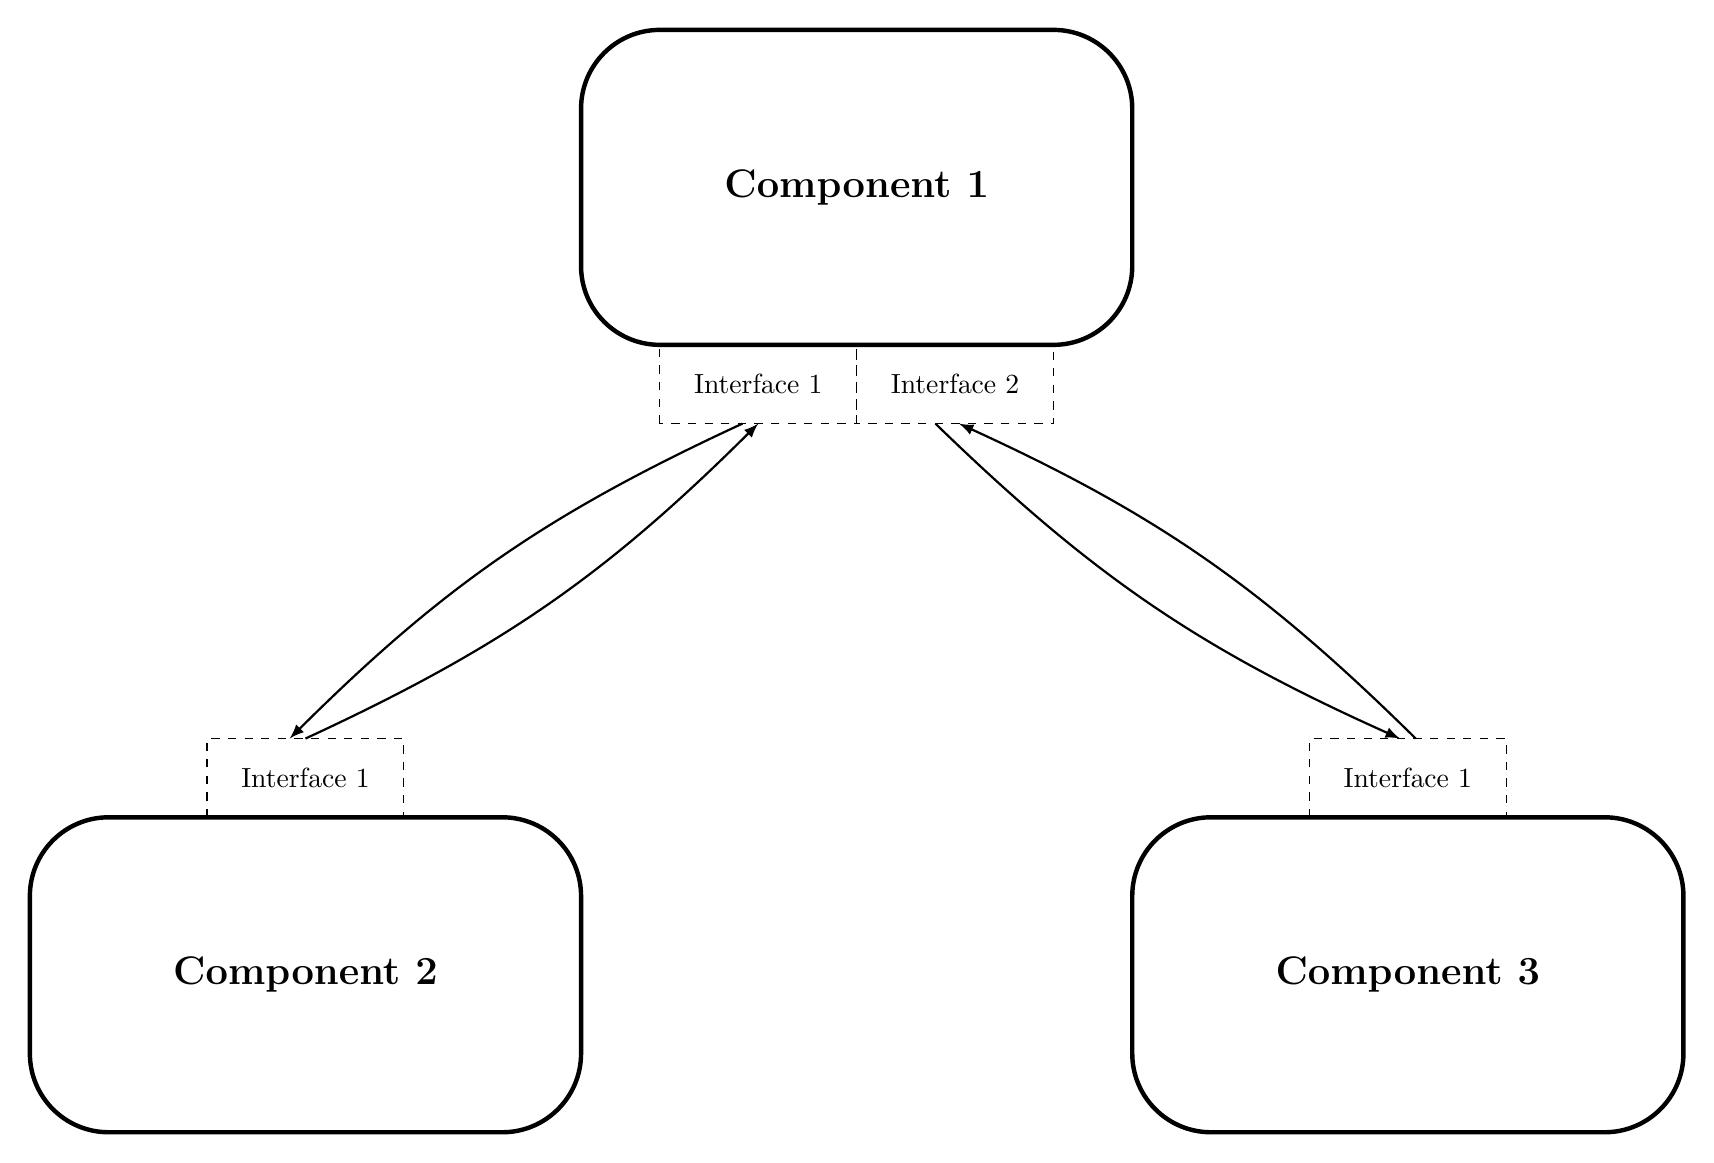
\begin{tikzpicture}


\draw [rounded corners=1cm,ultra thick] (0,0) rectangle ++(7,4) node [midway] {\Large\textbf{Component 1}};

\draw [dashed] (1,-1) rectangle ++(2.5,1) node [midway] {Interface 1};

\draw [dashed] (3.5,-1) rectangle ++(2.5,1) node [midway] {Interface 2};

\draw [rounded corners=1cm,ultra thick] (-7,-10) rectangle ++(7,4) node [midway] {\Large\textbf{Component 2}};

\draw [dashed] (-4.75,-6) rectangle ++(2.5,1) node [midway] {Interface 1};

\draw[-latex,thick] (-3.5,-5) to[bend right=10] (2.25,-1);

\draw[-latex,thick] (2.05,-1) to[bend right=10] (-3.7,-5);

%\draw[latex'-latex',ultra thick](-4,-5) to (2.25,-1);

\draw [rounded corners=1cm,ultra thick] (7,-10) rectangle ++(7,4) node [midway] {\Large\textbf{Component 3}};

\draw [dashed] (9.25,-6) rectangle ++(2.5,1) node [midway] {Interface 1};

\draw[-latex,thick] (10.6,-5) to[bend right=10] (4.8,-1);

\draw[-latex,thick] (4.5,-1) to[bend right=10] (10.4,-5);


\end{tikzpicture}}
    \caption{An abstract illustration of a CBA application of three components interacting via their interfaces.}
    \label{fig:cba_fig}
\end{figure}


\subsection{Challenges in Development of CBA Applications}
A CBA application consist of a topology of interconnected components, as shown in \autoref{fig:cba_fig}, where each component is responsible for some part of the overall system functionality. Individual components are built using traditional software engineering principles, which means that they are developed and tested in isolation before full-scale system integration and testing. Thus, errors usually occur due to the composition of the CBA application, where unforeseen states of component can cause them to fail \cite{Szyperski:2002:CSB:515228}. To find out which components failed during system integration, a technician usually has to go through the system logs generated during the testing in order to find the cause of failure. As this is a time consuming work for a technician, the aim is to automate this task. To get a better understanding of the challenges when trying to automate this task we now proceed to go through the structure of the system logs generated in the test suite environment. 

\section{System Logs}
System logs are generated in test suites, where all events executed are recorded in system log files. The structure of system logs we analyse in this thesis is presented in \autoref{fig:syslog_struct}.


\begin{figure}[H]
    \centering
        \begin{verbatim}
         
        Time_stamp Log_location process[PID]: Description
    
        \end{verbatim}
    \caption{The general structure of a system log.}
    \label{fig:syslog_struct}
\end{figure}

\noindent To understand each term of the system log we will go through them one by one.

\begin{itemize}[leftmargin=4em,align=left]
    
    \item \verb|Time_stamp| -- At which time the event was executed/logged.
    
    \item \verb|Log_location| -- The system log will either be logged in a \textit{system controller} or in a \textit{system Payload}, denoted \textit{SC} and \textit{PL} respectively.
    
    \item \verb|process| -- The name of the process that executed the command.
    
    \item \verb|[PID]:| -- The process identification, surrounded by brackets and ending with a colon.
    
    \item \verb|Description| -- States what occurred or action taken, and in some cases the severity level of the event.

\end{itemize}

\noindent The first three terms of the system log are rather self explanatory and thus we will not go into them any further. However, description is the term that is most important to solving the task of making the analysis of system logs autonomous. The description include information such as, severity, e.g. \textit{error} or \textit{rebooting}, effected components and their states, and sometimes a reason is stated. The challenge with the description is however that they do not follow a set of predefined rules, and are generally ill-structured. The reason for this is that each system log is written by a specific software engineering team who developed that component. Each software team or developer has their own unique style and selection of acronyms that becomes troublesome. Due to format and inconsistency of the description, it will impact the ability of the machine learning models to learn the patterns that separate the individual fault classes in the system logs. We have now introduced the general structure of the data set and we will now proceed to the theory of the machine learning model we will use.


To summarise this chapter; we started off by introducing the reason for component based software applications. Then, we briefly defined what a software component is and how it interacts with its environment. Next, we proceeded to state the challenges in the development of CBA systems. Finally, the general structure of the system logs was stated to get a context to the data set and its limitations.
%\chapter{The Neuroscience of the Neocortex}
\label{chp_neocortex}
This is a complementary chapter to \textit{''A Brain-Inspired Algorithm''}. We will go through some of the neuroscience of the \textit{new cerebral cortex} (neocortex), that the \textit{Hierarchical Temporal Memory} (HTM) theory is biologically derived from. We being by introducing the neocortex of the mammalian brain and why it is believed to be the part of the brain where intelligence resides. Then, the topology of the neocortex is presented, where we will go through the structure of each layer. Next, we describe the columnar organisation of the neocortex, first coined by Vernon B. Mountcastle, which is one of the main inspirations in HTM theory. We then continue to describe the neural circuitry of these cortical columns. Finally, we introduce the pyramidal neuron, which is the most frequently occurring type of neuron that resides in the neocortex. The HTM neuron is modelled on the pyramidal neuron's functionality and the active processing properties of its dendrites. 


\section{The Neocortex}
What separates all mammals from the rest of the animal kingdom is the existence of the neocortex in the cerebral cortex \cite{Neocortex}. The neocortex is perceived as the part of the brain where intelligence resides. The reason for this is that the neocortex is responsible for higher order brain functions, such as sensory perception, advanced motor control, association, memory, and cognition \cite{LodatoSimona2015GNDi}.  



\begin{figure}[ht!]
    \centering
    \begin{tikzpicture}
        \node[anchor=south west,inner sep=0] (image) at (0,0)
        {\includegraphics[scale=.35]{appendix/neuroscience/figures/brain2.png}};
        \node [anchor=west] (Neocortex) at (1,7) {Neocortex};
        \node [anchor=west] (Old Brain) at (3,1) {Old Brain};
            \begin{scope}[x={(image.south east)},y={(image.north west)}]
                \draw [-latex, thick, black] (Neocortex) to[out=0, in=120] (0.45,0.91);
                \draw [-latex, thick, black] (Old Brain) to[out=0, in=-120] (0.6,0.1);
            \end{scope}
    \end{tikzpicture}%
    \caption{\cite{BrainSketch} A sketch of the brain of a Homo sapiens. The cerebral hemisphere is recognised by the convoluted form with ridges and furrows.}
    \label{fig:forebrain}
\end{figure}


The forebrain, shown in figure \autoref{fig:forebrain}, is the largest part of the mammalian brain, made up of the cerebrum, thalamus, and hypothalamus. The cerebrum is made up of two cerebral hemispheres. The cerebral hemisphere has an outer layer of grey matter and the cerebral cortex beneath it \cite{crossman2014neuroanatomy}. The cerebral cortex consists of two areas, the neocortex and the allocortex, defined by their cytoarchitecture \cite{Allocortex}. The neocortex is larger in area and it is the outer most layer of the cerebral cortex, organised into six horizontal laminae of neurons. The allocortex is smaller in size with subareas such as the hippocampus, subiculum and olfactory cortex \cite{Neocortex}. Because mammals share the same brain structure of the olfactory cortex and the hippocampus with reptiles but not the neocortex, it was long viewed that the neocortex was a new evolutionary addition of the brain, hence the name. However, the neocortex should instead be viewed as homologous with the dorsal cortex of reptiles. Though, the difference between them is noticeable, the neocortex is a thick, laminated and uniform structure containing abundance of neurons; compared to the dorsal cortex in reptiles which contains only about a row of neurons in its sheet of tissue \cite{Neocortex}. With these dissimilarities in mind, the function of all vertebrate brains is still the same, which is to act as a premotor organ that sends motor commands to the animals' muscles \cite{10.3389/fnana.2013.00051}. 


What makes the human neocortex so special that its able to give us humans the ability to express our thoughts through motor commands, e.g. writing or speaking, perception, imagination, language processing and cognition? One major factor to why humans surpasses it counterparts in intelligence is the sheer size of the neocortex, a surface area of roughly 2600 cm$^2$ and a thickness of 3-4 mm, together with the vast number of neurons, up to $28\times10^9$, that resides there \cite{MountcastleVernon1997}. The human neocortex wraps around the forebrain in a convoluted fashion, compared to a rodents' neocortex which is non-folded. This allows the human neocortex to have more surface area with a limited volume \cite{folded}. Another reason why humans surpasses all other mammals is evolutionary, i.e. having a large neocortex with many subdivisions is metabolically costly, takes a long time to develop and mature and is unnecessary for most other animals \cite{Neocortex}. 


\subsection{The Topology}
The neocortex organized in hierarchy of six horizontal stacked laminae, numbered I--VI, with each of the layers grouped based on synaptical connectivity, morphological type of neurons and at which depth they exist \cite{Neocortex}. This basic structure is shown in \autoref{fig:layers}. To understand the difference of each layers' topology and processing properties, a brief description is given below:



\begin{itemize}[leftmargin=4em,align=left]
    \item \textbf{Layer I:} The top layer, which is mostly inhabited by fibers that run parallel to the surface. The fibers consist of the ends of apical dendrites and axons that connect to each other via synapses, together with a few neurons. This layer serves two purposes; first, to work as a feedback connection from other cortical areas. Secondly, to modulate input from the brain stem \cite{Neocortex}.
    
    \item\textbf{Layer II:} This layer has a large population of small neurons. The dendrites of these neurons are connected to neighbouring cortical areas and pyramidal neurons in deeper layers via their apical dendrites. Thus, allowing intracortical connections to affect the processing in a local area \cite{Neocortex}.
    
    \item\textbf{Layer III:} One of the main output layers of the neocortex, consisting of medium sized pyramidal neurons with basal and apical dendrites. The axons of these neurons serves as commissural fibers, i.e. connections between the two cortical hemispheres, and as connections to other cortical areas \cite{crossman2014neuroanatomy}. The pyramidal neurons receive their input form other layers in the local area via their apical dendrites. Adjacent neurons in layer III are able exchange information via their basal dendrites. This layer is of great importance, as it makes it possible for information exchange between regions in the neocortex. Thus increasing the complexity of possible operations that can be performed \cite{Neocortex}.
    
    \item\textbf{Layer IV:} The main input layer and situated in the middle occupied by small stellate cells. The name is given due to the radial propagation of the dendrites. The information that the stellate cells receives is shared locally between neighbours via the basal dendrites and then transmitted to the adjoining layers above and below. The stellate cells are small due to the fact that the axons and dendrites only extend a short range \cite{Neocortex}.
    
    
    \item\textbf{Layer V:} This is the other main output layer of the neocortex. Large pyramidal neurons inhabit this layer, which can be seen in \autoref{fig:layers} as triangular black spots. The main task of this layer is to integrate information from both its horizontal neighbours and all vertically connected neurons in the layers above up till layer I that belongs to the same cortical column \cite{Neocortex}. This information is then sent out to extra-cortical parts of the brain, i.e. basal ganglia, thalamus, brain stem and the spinal cord, via long axons \cite{crossman2014neuroanatomy}. But also to remote cortical areas, including areas in the other cerebral hemisphere. As these distances can be quite far and information needs to travel fast, the axons needs thick, as this allows for faster conduction rates. To gather information from the vertically adjoining layers, the apical dendrites branch out in long vertical fibers, with synaptic connections in each layer. Neighbouring cells communicate via their basal dendrites. For the pyramidal neurons to be able to send and receive action potentials on their long apical dendrites, and also thick axons the cell body needs to be large \cite{Neocortex}.
    
    
    \item\textbf{Layer VI:} Until this layer, the information has just been processed in a feed-forward manner, i.e. receive information, manipulate it and transmit it onward to other regions. But bi-directional communication is necessary in any complex computational unit, and this is where layer VI comes in. This is the main feedback layer to other activation regions about the state of the local area. The pyramidal neurons that resides in layer VI mainly get their input for layer IV, as well as direct input from axons that terminate in layer IV. With these connections, layer VI is able to project back information to the neurons in another cortical area that contributed to the activation \cite{Neocortex}. 
    
    
\end{itemize}

\begin{figure}[H]
    \centering
    \includegraphics[scale=.88]{appendix/neuroscience/figures/layers.jpg}
    \caption{\cite{IVIlayers} The cross section above, visualises the general structure of the neocortex categorised into six horizontal laminae, I--VI, on the basis of cytoarchitecture. The cell bodies of the neurons are shown as the darkened spots, neither the axons nor dendrites of the neurons are visible. The white matter connects the neocortical region to other regions in the neocortex along with other parts of the brain. These connections allows the region to send and receive signals \cite{Neocortex}.}
    \label{fig:layers}
\end{figure}

\noindent With the understanding of each layers' properties we can now move on to explain the most basic processing unit of the neocortex, the \textit{minicolumn} and the \textit{cortical column}.

%COLUMNAR ORGANISATION
\subsection{Columnar Organisation}
The most basic processing unit in the neocortex is called a \textit{minicolumn}, first described by Vernon B. Mountcastle in 1955--1959 \cite{doi:10.1093/cercor/13.1.2}. A minicolumn is a vertical array of neurons connected to each other like a chain across layer II--VI. These minicolumns have transverse diameter of 50--80 $\mu$m and contain between 80--100 neurons in primates, but can contain up to 2 times more in the striate cortex. The structure of the minicolumn can be observed throughout the neocortex, however they are not identical as some features differ, e.g. cell phenotypes, synaptic transmitters \cite{doi:10.1093/cercor/13.1.2}. A \textit{cortical column} is a group of minicolumns which is formed by a common input and the horizontal links they have with each other. The number of minicolumns that a cortical column contains varies between 50--80 \cite{doi:10.1093/cercor/13.1.2}. The cortical column functions as a complex distributed system, where each minicolumn can be viewed as a computing node, which is able to modulate inputs and use bilateral communication with neighbouring minicolumns and cortical columns. This allows the cortical columns to link multiple inputs to multiple outputs \cite{MountcastleVernon1997}.


\subsection{Neural Circuit Functionality}
In each minicolumn there exists two types of neurons; the \textit{excitatory neurons}, i.e. pyramidal and spiny stellate cells; and the \textit{inhibitory neuron}, the aspiny stellate cells. The neurons are distributed throughout the layers in the minicolumn with the majority, $\sim$80\% , of the neurons being of the excitatory type \cite{Neocortex}. The excitatory neurons are able to depolarise the neurons of which it is synaptically connected to by sending out a excitatory neurotransmitter, glutamate. In this depolarised state the effected neuron is more likely to itself send out an action potential if it receives strong enough signal on its dendrites \cite{Neocortex}. The opposite is true for the inhibitory neuron, as it sends out an inhibitory neurontransmitter, i.e. a biochemical called \textit{gamma-Aminobutyric acid}, or GABA, which hyper-polarises the effected neuron, making it less likely to produce an action potential. This inhibitory effect allows a local circuit to remain sparse, as minicolumns that respond to the same input tend to inhibit each other. This limits the response time for an input and makes the cortical column sensitive to temporal changes \cite{Neocortex}. 


 The cortical columns are able to correlate different inputs based on interconnections that exist in layer III, as these makes horizontal connection in between cortical columns. The advantage of such connections are that neurons in different cortical columns can become active at the same time, thus being able to respond to the signal of the same object and giving it cohesion \cite{Neocortex}. Another crucial part of the neural circuits is its plasticity. The synaptic connections between neurons change over time, either they become stronger or weaker, which makes the brain able to adapt to new input. This is largely due to the two types of membrane receptors that exist, i.e. the \textit{N-methyl-D-aspartate}, or NMDA, receptor and the non-NMDA receptor. The non-NMDA receptor reacts when glutamate is released, which leads to depolarisation of a neuron. When this happens, the NMDA receptor, which is otherwise blocked by magnesium ions, is unblocked and can pass calcium ions through if another glutamate release occurs in a short amount of time. This leads to a fast succession of action potential being generated by the neuron. Because of this, synaptic strength between the the neurons is increased, which is called long-term potentiation. The opposite is called long-term depression, which means that the neurons does not respond to the same input and their synaptic connections are weakened \cite{Neocortex}. This alteration of the synaptic strength between neurons is also known as Hebbian learning \cite{CapaldiE.John1992TOOB}. 
 
 It is in these synaptic connections that memories are stored. Memories are stored in a sequences and can be recalled auto-associatively. This makes the neocortex robust to noise and incomplete input patterns, as it can auto-complete as input patters as memories are recalled in an ordered sequence. Thus, the neocortex is able to make predictions about the future based on incomplete input \cite{memory}. 

\section{Pyramidal Neuron}
\label{sec:dendrite}
The most abundant of all neuron types in the neocortex is the pyramidal neuron. The pyramidal neuron is unique to the cerebral cortex and can be found in all layers except the first and represent between 70-85\% of the total population in any cortical area. It has therefore been seen as the principle neuron of the cerebral cortex \cite{PyramidalPop}. As the name indicates, the cell body, or \textit{soma}, of the pyramidal neuron has a pyramidal shape, which can be seen in \autoref{fig:pyramidal}.


\begin{figure}[ht!]
    \centering
    \includegraphics[scale=.3]{appendix/neuroscience/figures/PyramidalNeuron.png}
    \caption{\cite{PyramidalPop} A sketch of a stereotypical pyramidal neuron, with a apical dendrite branching out from the apex of the soma, the basal dendrites extends out in the horizontal direction and the axon is descending from the soma.}
    \label{fig:pyramidal}
\end{figure}


\subsection{Dendrites, Synapses and Axons}
The \textit{dendrites} are the input branches of a neuron, which is either able to excite or inhibit the neuron based on the neurotransmitter it receives on its \textit{synapses}. The synapses are the connections between the output branches, or \textit{axons}, and the dendrites, that allows electrical or chemical signal to be transmitted. An axon is the main output branch of the neuron, and is able to transport the signal, or action potential, to its synapses. In the dendrites the input signals are integrated, which in turn changes the state of the neuron if a complex set of conditions are met. Firstly, the integrated signal at a spatial position on the dendrite branch needs to exceed a threshold. This threshold is dynamic as the integrated signal needs to be stronger if its further away from the soma. The second condition that needs to be met is the timing of the synaptic conductances that occur at the integration zone \cite{PyramidalNeuron}. The dendrites can be classified into three zones, the \textit{basal}, \textit{proximal} and \textit{distal} zone. The basal zone contains the basal dendrites that extend along the horizontal axis and connect to neighbouring neurons in the cortical column. The apical dendrite can be divided into two parts, a proximal zone, closer to the soma, and the distal zone which is further away. In the distal zone the amplitude of the integrated signal needs to be higher in order to effect the cell state, due to the longer travel distance. The pyramidal neuron is believed to act as a coincidence detector as its been shown to respond best to simultaneous stimulation in distal and proximal areas of the apical dendrite \cite{PyramidalNeuron}. Another important feature of the pyramidal neurons is its ability to adapt to change in the temporal input patterns. It able to change functionality due to synaptic plasticity, which is ability to change the strength of the synaptic connection between neurons \cite{PyramidalNeuron}. As explained in the previous section, the strength of the synaptic connections alters with long-term potentiation or long-term depression.

\section{Summary}
To summaries, HTM theory is derived from properties of the neocortex and the ideas of Vernon B. Mountcastle's single cortical algorithm for information processing. This chapter aimed to familiarise the reader with the structure and functionality of neocortex. First, a gentle introduction to the neocortex was given. Then, we proceeded to the topology and the structure of the individual layers. Next, cortical columns and the neural circuitry was presented, which HTM theory tries to reverse engineer to some extent. Finally, we presented the pyramidal neuron and the functionality of the dendrites. As this is the most abundant neuron in the neocortex, and the inspiration of the HTM neuron's functionality.





%To achieve true machine intelligence one must first be able to understand the information processing that occurs in the brain. Some AI researchers have discarded the idea of this principle with the argument that neither planes nor cars function in the same way as their biological counterparts \cite{Hawkins:2004:INT:993636}. However, intelligence should be defined as the methodology by which an autonomous agent is able to learn in the world \cite{Intelligence}. This means that intelligence resides in the inner workings of the brain and is not equivalent to behaviour. With this definition of intelligence; current state-of-the-art AI agents that can outperform humans in some specific tasks, such as image classification or Go, cannot be seen as intelligent. 



%Geoffrey Hinton, who is hailed as one of the godfathers of Deep Learning is ''deeply suspicious'' of the learning algorithm of Artificial Neural Networks called Back-Propagation, and encourages graduates to scrap this idea and explore new possibilities of learning for neural networks \cite{Hinton}.

%The goal of AI research is to create a Artificial General Intelligence that is on par or surpasses human intelligence. But what makes the human brain so special? It is the size of the \textit{new cerebral cortex} (neocortex) \cite{Neocortex}.
\chapter{A Brain-Inspired Algorithm}
\label{chp_htm}
\textit{Hierarchical Temporal Memory} (HTM) is a theory of how the human neocortex processes information, be it auditory, visual, motor, or somatosensory signals, developed by Jeff Hawkins \cite{Hawkins:2004:INT:993636}. It was long known that the neocortex looked remarkably similar in all different regions, this made anatomists to focus on the minuscule differences between the cortical regions to find the answer how they worked. However, in 1978, a neuroscientist by the name of Vernon B. Mountcaslte stopped focusing on the differences and saw that it was the similarities of the cortical regions that mattered. He came up with a theory of a single algorithm by which the neocortex processes information. The small differences that the anatomists found, was only because of the different types of signals that where being processed, not a difference in the algorithm itself \cite{Hawkins:2004:INT:993636}. With this idea of a single algorithm, Jeff Hawkins started a company called Numenta, with the intention of figuring out this algorithm. Numenta has since published an open-source project named Numenta Platform for Intelligent Computing, or NuPIC, which is an implementation of the HTM theory. 

In this chapter, we will start by introducing the HTM neuron. Then, we proceed to explain the way information is represented in an HTM network. Finally, we explain the sequence learning algorithm, called temporal memory.


\section{HTM Neuron Model}
The HTM neuron model is an abstraction of the pyramidal neuron in the neocortex \cite{10.3389/fncir.2016.00023}. However, so is the point neuron, which is used in most \textit{Artificial Neural Networks} (ANNs); so how different are they? The point neuron, see \autoref{fig:pointNeuron}, summates all the inputs on its synapses, then passes this value through a non-linear activation function. If the output value is above a threshold, the neuron outputs the value of the activation function; otherwise it will output a zero. With the properties of the dendrites explained in \autoref{sec:dendrite}, one could argue that point neurons does not have dendrites at all, and therefore completely lack the active properties of the dendrites. 


The connection between the point neurons is instead the synaptic connection, which can be changed via back propagation \cite{LeCunYann2015Dl}. 

\begin{figure}[ht!]
    \centering
    \input{background/HTM/tikz/pointNeuron.tex}
    \caption{The point neuron, used in most ANNs, summates the synaptic input and passes in through an activation function. It lacks active dendrites and only has synaptic connections.} %\cite{ANtikz}
    \label{fig:pointNeuron}
\end{figure}


The HTM neuron, see \autoref{fig:HTMNeuron}, is modelled on the active dendrite properties, and is therefore able to make use of the coincidence detection of the pyramidal neuron. The coincidence detection is activated via non-linear integration when a small number of synapses, experimentally show to be around 8-20, are active in close spatial proximity on a dendritic segment \cite{10.3389/fncir.2016.00023}. This non-linear integration will cause an NMDA dendritic spike, thus allowing the neuron to recognise a pattern \cite{10.3389/fncir.2016.00023}. In order for the neuron to be able to recognise a vast number of different patterns, the active input pattern needs to be sparse, i.e. only a few neurons that are active per input pattern. If we assume that the total number of neurons in a population is $n$, and at any given time the number of active cells are $a$, then sparse activation is given as $a \ll n$. On each dendritic segment there are $s$ number of synapses. For a dendritic segment to release an NMDA spike, the number of synapses that needs to be active is $\theta$, i.e. the NMDA spike threshold, of the total number of synapses $s$ \cite{10.3389/fncir.2016.00023}. By forming more synaptic connections for each pattern than necessary the neuron becomes more robust to noise and variation in the input pattern. However, the trade-off in these extra connections is the increased likelihood of the neuron to classify false positives, but if the patterns are sparse the increased likelihood is infinitesimal \cite{10.3389/fncir.2016.00023}. The dendrites can be divided into three zones of synaptic integration, the \textit{basal}, \textit{proximal}, and \textit{distal zone} \cite{10.3389/fncir.2016.00023}. These zones are categorised based on input and spatial position on the neuron, and are explained below.

\begin{figure}[ht!]
    \centering
    \hbox{\hspace{3.5em}\input{background/HTM/tikz/HTMNeuron.tex}}
    \caption{The schematic of the HTM neuron with arrays of coincident detectors consisting sets of synapses. However, in this figure only a few is shown, where black dots represents active synapses and white inactive ones. An NMDA spike is generated if the total number of active synapses are above the NMDA spike threshold, $\theta$, (represented as a Heaviside node) on any of the coincident detectors in a dendritic zone, which is represented by OR-gate. The dendritic zones can be divided in to three different zones base on the distance from the soma and synaptic connections. The proximal dendrites receive the \textit{feedforward} pattern, also know as the receptive field of the neuron. The basal zone receives information about the activity of neighbouring neurons of which its connected to and can be seen as giving \textit{context} to the input pattern. Apical dendrites receive the \textit{feedback} information form the layers above which also can effect the state of the soma \cite{10.3389/fncir.2016.00023}.}
    \label{fig:HTMNeuron}
\end{figure}



\subsection{Proximal Zone}
The feedforward input is received by the dendrites in the proximal zone, as this is the main receptive field of HTM neuron \cite{10.3389/fncir.2016.00023}. The proximal zone is the dendritic zone closest to the soma, usually consisting of several hundreds of synapses. Because of the proximity to the soma, the NMDA spike generated in this dendritic zone is strong enough to effect the soma in such a way that it generates an action potential. If the input pattern is sparse, subsets of synapses are able to generate NMDA spikes. Therefore, the coincident detector can detect multiple different feedforward patterns in one input signal, thus it can be viewed as a union of several unique patterns \cite{10.3389/fncir.2016.00023}.


\subsection{Basal Zone}
The basal zone is the dendritic segment that connects neuron in different minicolumns to each other. These connection allow a neuron to detect activity of neighbouring neurons, which enables individual neurons to learn transitions of input patterns. When a basal segment recognises a pattern, it will generate an NMDA spike. But due to the distance from the soma, the signal attenuates and is not able to generate an action potential in the soma. However, it does depolarise the soma, also called the \textit{predictive state} of the neuron. The \textit{predictive state} is an important state of the neuron because it has major contribution to the overall network functionality. If a neuron is in the predictive state it will become active earlier than its neighbours, in the same minicolumn and close proximity, if the feedforward pattern activates the proximal segment. When a neuron transitions from the predictive state to the active state it will not only give of an action potential, but also inhibit its neighbours from becoming active. Thus, keeping the activation pattern for recognised input patterns sparse \cite{10.3389/fncir.2016.00023}. This type of inhibition of nearby neurons is a way to represent the functionality of inhibition neurons, without representing them as individual cells \cite{10.3389/fncir.2017.00081}.


\subsection{Distal Zone}
Furthest from the soma is the apical dendrites, which connects neurons to the ascending layers. Much like the basal dendrites, apical segment does not generate a signal strong enough to cause an action potential in the soma. The signal generated on the apical segment differs from the signal generated on the basal segment. When a pattern is recognised, the NMDA spike does not directly travel to the soma. Instead, the soma is depolarises by a calcium ion, Ca$^{2+}$, spike generated at the dendritic segment. This depolarisation gives the neuron a ability of doing top-down extraction \cite{10.3389/fncir.2016.00023}.


\subsection{Learning}
The learning of an individual HTM neuron is based on two principles; formation and removal of synaptic connection via Hebbian style learning \cite{10.3389/fncir.2016.00023}. Each dendritic branch has a set of potential synaptic connection, where each connection can become active if there is enough simultaneous activity between the two potentially connected neurons. For a dendritic branch to recognise a pattern there needs to be a subset of the connected synapses that are active. This threshold is usually set to 15-20 \cite{10.3389/fncir.2016.00023}. When a dendritic branch becomes active, the entire dendritic segment is seen as active to the neuron, which is visualised in \autoref{fig:HTMNeuron} by the OR gate. The HTM neuron learns to detect new pattern by forming new synaptic connection on a dendritic branch. Each potential synaptic connection is given a \textit{permanence} value, which determines the strength of a synaptic connection between the neuron's dendritic branch and another neuron's axon in the network. The permanence value is defined on the range $[0, 1]$, where $0.0$ means that there is no connection, and $1.0$ means that a fully formed synapses has been grown. The potentiation and depression of each permanence value is achieved via a Hebbian learning rule, i.e. if neurons fire together they wire together. In order for a synaptic connection to be formed, the permanence value has to be above a certain threshold, e.g. $0.3$. With a permanence value above the threshold, the synaptic weight is assigned to 1 between the neurons. Therefore, there is no difference if the permanence value is $0.3$ or $1.0$ when a pattern is recognised. However, the lower the value is, the easier it is for the neuron to forget the connection, and in extension the pattern. With this growing mechanism of the neuron, the tolerance to noise and on-line learning is possible \cite{10.3389/fncir.2016.00023}. 





\section{Information Representation and Detection}
\subsection{Sparse Distributed Representation}
The presynaptic input patterns of information that is received by the dendrites, needs to be robust to noise and have a vast encoding capacity, as the neocortex handles an endless stream of sensory input. Empirical evidence shows that the neocortex operates by using sparse representations of information \cite{DBLP:journals/corr/AhmadH16}. In HTM theory, these sparse activation patterns are called \textit{Sparse Distributed Representation}, or SDR. Sparseness is due to the low number of active neurons at any given time, and it is distributed as no information is encoded in a single neuron. The information of the cell activity that the dendrite receives from the presynaptic cells is either active or non-active, and can therefore be modelled as a binary vector \cite{DBLP:journals/corr/AhmadH16}. 


\begin{figure}[ht!]
    \centering
    \resizebox{\textwidth}{!}{\input{background/HTM/tikz/sdr_fig.tex}}
    \caption{An example of an SDR, where black squares represent active cells and white squares represent inactive ones. The SDR is represented as matrix for convenience.}
    \label{fig:sdr_ex}
\end{figure}


In \autoref{fig:sdr_ex}, we present an example of presynaptic input, or SDR, represented as a bit vector. Each cell can either be active or inactive, represented as black and white squares respectivly. The entire presynaptic input space of $n$ cells, at time $t$, for a dendritic segment is represented by an $n$-dimensional SDR, $\boldsymbol{X}_t$:


\begin{equation}
    \boldsymbol{X}_t = [b_0,\ b_1,...,\ b_{n-1}]
\end{equation}


\noindent where $b_i \in \mathbb{Z}_2$. The number of active cells is given by $w_X = | \boldsymbol{X}_t |$ and the pattern is considered sparse if $w_X \ll n$. The number of possible encodings the presynaptic input pattern is given by:


\begin{equation}
    \begin{pmatrix} n \\ w_X \end{pmatrix} = \frac{n!}{w_X!(n-w_X)!}
\end{equation}


\subsection{Presynaptic Pattern Detection}
A dendritic segment can also be modelled as a binary vector $\boldsymbol{D}$ of length $n$, which represents both potential and established synaptic connections to the presynaptic input. The active synaptic connections are represented as the non-zero elements, where $b_i$ is the synaptic connection to the presynaptic cell $i$. The number of established connections, represented by $s = | \boldsymbol{D} |$, has been experimentally shown to typically be around 20 to 300 synapses for a dendritic segment. But the potential connections can be in the thousands \cite{DBLP:journals/corr/AhmadH16}. To generate a spike in a dendritic segment, the number of synaptic connections that receive active input form the presynaptic cells needs to exceed a threshold, $\theta$. This threshold can be computed via the dot product of the two binary vectors:

\begin{equation}
    m(\boldsymbol{X}_t,\boldsymbol{D}) \equiv \boldsymbol{X}_t \cdot \boldsymbol{D} \geq \theta
\end{equation}


Where the threshold usually is lower than the number of connections and presynaptic activity, i.e. $\theta \leq s$ and $\theta \leq w_X$. As $\boldsymbol{X}_t$ does not represent the full presynaptic input pattern, but only a subsample, each dendritic segment only learns synaptic connections to some active cells of the entire pattern. How well a dendritic segment detects a pattern is dependent on the value of the NMDA spike threshold, $\theta$, and the robustness to noise in SDR encodings. With lower values of $\theta$ the dendritic branch is able to detect known input patterns easier. However, there is an inherent trade-off in small values of $\theta$, as the dendritic branch are then more likely to detect false positives if there is noise in the input pattern \cite{DBLP:journals/corr/AhmadH16}. 

If $\theta$ is set to a reasonable value, e.g. around 8-20, the probability of false detection due to noise in the SDR will be extremely unlikely. The reason for this is the sheer size of possible combination of ON-bits in the SDR. SDRs corrupted by some noise will not overlap enough to been interpreted as another possible input pattern. Therefore, detection on each dendritic segment with inexact matching has a very low probability of false detection, as described by Ahmad et al. in \cite{DBLP:journals/corr/AhmadH16}.


In each cortical region there are millions of neurons that simultaneously trying to recognise hundreds of patterns. They are able to recognise hundreds of patterns, as there only needs to be between 8 to 20 active synapses to generate an NMDA spike. On each of these neurons there are numerous dendritic branches, that combined have several thousands of synapses on them. Therefore, the robustness of the single dendritic segment needs to be maintained throughout a large neuron network \cite{DBLP:journals/corr/AhmadH16}. 


To quantify the robustness properties in the a larger scale we will first introduce the probability of false positives for an arbitrary number of dendritic segments, of which do not have to belong to the same neuron. Let $M$ be the number of different patterns represented by $M$ different dendritic segments, all of which has the threshold $\theta$ and $s$ number of synapses. The set of the dendritic segments is given by $S = \{ \boldsymbol{D}_0,\ \boldsymbol{D}_1,\ ...,\ \boldsymbol{D}_{M-1}  \}$, where $\boldsymbol{D}_i$ represents a dendritic segment vector. Let $\boldsymbol{X}_t$ be a random presynaptic input, of which is classified as belonging to the set if the following is true:


\begin{equation}
    \boldsymbol{X}_t \in S\ :=\ \exists_{\boldsymbol{D}_i}\ m(\boldsymbol{D}_i, \boldsymbol{X}_t) = True
\end{equation}


There is no false negatives if the number of corrupt bits in $\boldsymbol{X}_t$ is $\leq w_{D_i} - \theta$. The probability of a false positive is given by:

\begin{equation}
    P(\boldsymbol{X}_t \in S) = 1 - (1-P(m(\boldsymbol{X}_t, \boldsymbol{D}_i)))^M
\end{equation}

Which computationally difficult to compute as the probability of individual overlap is extremely unlikely \cite{DBLP:journals/corr/AhmadH16}.

\subsection{The Union Property on Dendritic Segments}
Another important property that comes with the SDR encoding is the ability to group and reliably store a set of SDR with a single SDR representation. This is achieved by taking the union of all the SDRs in a set, and is called the \textit{union property} \cite{DBLP:journals/corr/AhmadH16}. For binary vectors this is equivalent to taking the Boolean OR between all vectors. The ability to store multiple patterns is an important feature of the dendritic segment. In dendritic segments the synapses that respond to different patterns are stored in the same SDR. Thus, multiple presynaptic patterns can cause an NMDA spike to be generated. For a dendritic segment, $\boldsymbol{D}$, to be able to detect an arbitrary number of $M$ synaptic SDRs, we simply take union of all individual synaptic connection vectors, $\boldsymbol{d}_i$:

\begin{equation}
    \boldsymbol{D} = \bigcup_{i=0}^{M-1} \boldsymbol{d}_{i}
\end{equation}


The patterns will be detected as long as $\theta$ number of synapses are active. By increasing the $M$, the number of patterns that a dendritic segment can detect increases, but so does the probability of false detection. Therefore, there is a limit to the amount of ON-bits a dendritic segment can have, before the detection of false positives becomes a problem \cite{DBLP:journals/corr/AhmadH15}. Using unions, we are able to make temporal predictions, temporal pooling, create invariant representations, and create an effective hierarchy \cite{DBLP:journals/corr/AhmadH15}.








\begin{comment}
To prove the robustness to high levels of noise of the SDR encoding, $\boldsymbol{X}$, of $n$ presynaptic cells, we first need to explain the notion of \textit{overlap sets} and then \textit{inexact matching} \cite{DBLP:journals/corr/AhmadH16}. The overlap set allows us to examine the set of vectors of size $n$, that has $a$ ON-bits of which $b$ ON-bits overlap with $\boldsymbol{X}$. The number of vectors that belong to this set is defined as $\Omega_{\boldsymbol{X}}(n,a,b)$. Under the condition that $b \leq |\boldsymbol{X}|$ and $b \leq a$ we can compute the cardinality of this subset of vectors by: 

\begin{equation}
    |\Omega_X(n,a,b)| = \begin{pmatrix} |\boldsymbol{X}| \\ b \end{pmatrix} \times \begin{pmatrix} n - |\boldsymbol{X}| \\ a - b \end{pmatrix}
\end{equation}

\noindent Where the first term represents the number possible subsets of $\boldsymbol{X}$ that share $b$ on-bits, and the second term is all the patterns with $n - |\boldsymbol{X}|$ bits, of which the number of on-bits are $a - b$. Inexact matching allows us to give the probability that a dendritic segment, $\boldsymbol{D}$, will detect a random presynaptic activation pattern, $\boldsymbol{X}_t$  \cite{DBLP:journals/corr/AhmadH16}. The probability is given by the number of possible patterns that the dendritic segment can detect, divided by the number of possible activation patterns.

\begin{equation}
   P(m(\boldsymbol{X}_t, \boldsymbol{D}))  = \frac{\sum^{s}_{b=\theta}|\Omega_{\boldsymbol{D}}(n,w_X,b)|}{\begin{pmatrix} n \\ w_X \end{pmatrix}}
\end{equation}

This gives the probability of a false match for a given dendritic segment \cite{DBLP:journals/corr/AhmadH16}. If the presynaptic input pattern, $\boldsymbol{X}_t$, is corrupted by noise such that $v$ of the on-bits are now off, represented as $\boldsymbol{X}^{\prime}_t$, there is a probability of false negatives. The probability of a false negative increases with $v$, such that $\boldsymbol{X}^{\prime}_t \cdot \boldsymbol{D} < \theta$. As the overlap has to go below the threshold, there is no possibility of a false match if $v$ is sufficiently small, i.e. $v \leq s - \theta$. The computation of the probability of a false negative computed in a similar fashion to false positives \cite{DBLP:journals/corr/AhmadH16}. But instead of we have the cardinality of overlap set of $\boldsymbol{X}^{\prime}_t$ with respect to $\boldsymbol{D}$ in the numerator:

\begin{equation}
    |\Omega_{\boldsymbol{D}}(w_{X^{\prime}},v,b)| = \begin{pmatrix} s \\ b \end{pmatrix} \times \begin{pmatrix} w_{X^{\prime}} - s \\ v - b \end{pmatrix}
\end{equation}

\noindent And thus the probability of a false negative is given by:

\begin{equation}
   P(\boldsymbol{X}^{\prime}_t \cdot \boldsymbol{D} < \theta)  = \frac{\sum^{s}_{b=s - \theta + 1}|\Omega_{\boldsymbol{D}}(w_{X^{\prime}}, v, b)|}{\begin{pmatrix} w_{X^{\prime}} \\ v \end{pmatrix}}
\end{equation}

\end{comment}


\section{Temporal Memory}
\label{sec:TM}
\subsection{Notation}
The sequence learning algorithm of the HTM theory is called the \textit{temporal memory} \cite{10.3389/fncir.2016.00023}. The temporal memory consists of a layer of $N$ mini-columns stacked vertically. Each mini-column contains $M$ number of HTM neurons, thus a total of $NM$ cells. The cells can be in one of three states; active, non-active, or predictive (depolarised). Thus, for a given time-step, $t$, the active cells in the layer are represented by the $M \times N$ binary matrix, $\boldsymbol{A}^{t}$, where $a^{t}_{ij}$ is the current active (non-active) state of the $i$'th cell in the $j$'th minicolumn \cite{10.3389/fncir.2016.00023}. For the same time-step, the predictive state of each cell is given by the $M \times N$ binary matrix, $\boldsymbol{\prod}^{t}$, of which the predictive state of the $i$'th cell in $j$'th minicolumn is denoted by $\pi^{t}_{ij}$ \cite{10.3389/fncir.2016.00023}.


Each cell in a layer has the potential to connect to any other cell via its basal dendrites. The set of basal dendritic segments of the $i$'th cell in $j$'th minicolumn is therefore represented by $\boldsymbol{D}_{ij}$. Each segment has a subset of $s$ potential synaptic connections from the $NM - 1$ cells in the layer. This subset is associated with a non-zero permanence value, where the $d$'th dendritic segment is represented as a $M \times N$ sparse matrix, $\boldsymbol{D}^{d}_{ij}$. A synaptic connection is only considered to be established if the permanence value is above a certain threshold. To represent these synapses with a weight of 1 on the same dendritic segment, we have the following $M \times N$ binary matrix, $\tilde{\boldsymbol{D}}^{d}_{ij}$ \cite{10.3389/fncir.2016.00023}.

\subsection{Initialisation of the Dendritic Segments}
With the initialisation of the network, each cell's dendritic segments are randomly assigned unique sets of $s$ potential synaptic connections. The non-zero permanence value of these connections is randomly initialised, with some being above the threshold and thus being connected, while others are not and therefore are unconnected \cite{10.3389/fncir.2016.00023}.

\subsection{Activation of Cells}
Each minicolumns feedforward receptive field is a subset of the entire feedforward pattern \cite{10.3389/fncir.2016.00023}. The receptive field of a minicolumn is shared by all cells in that minicolumn. A minicolumn becomes active if the number of synapses connected to the receptive field is above a certain threshold. However, there is an upper bound of $k$ minicolumns that can be active at the same time. Thus the minicolumns that have the highest number of active synapses get selected, which is also called the inhibitory process \cite{10.3389/fncir.2016.00023}. The set of $k$ winning minicolumns is denoted by $\boldsymbol{W}^{t}$. The active state of the individual cells in each minicolumn is computed by:


\begin{equation}
    a_{ij}^{t} =
    \begin{cases}
      1,&\text{if } j \in \boldsymbol{W}^{t} \text{ and } \pi^{t-1}_{ij} = 1\\
      1,&\text{if } j \in \boldsymbol{W}^{t} \text{ and } \sum_i\pi^{t-1}_{ij} = 0\\
      0,&\text{otherwise}
    \end{cases}
\end{equation}


In the first case the cell will become active if it was in a predictive state in the time-step before. In the second case, all cells in a minicolumn will become active if none of them previously where in a predictive state. If none of these cases applies, the cell will remain inactive \cite{10.3389/fncir.2016.00023}. Next, the predictive state of each cell in the winning column is computed as follows:


\begin{equation}
    \pi^{t}_{ij} = 
        \begin{cases}
            1,&\text{if } \exists_d\ \Big\| \tilde{\boldsymbol{D}}^{d}_{ij} \circ \boldsymbol{A}^{t} \Big\|_1 > \theta\\
            0,&\text{otherwise}
        \end{cases}
\end{equation}


For a cell to become depolarised in the current time-step, the contextual information received from the presynaptic input on any basal dendritic segment needs to be above the NMDA spike threshold, $\theta$. In order to detect if a segment is above this threshold, an element-wise multiplication, represented by $\circ$, of the dendritic segment and the active cells in the layer is computed. The $L_1$-norm of the result is then computed and compared with the threshold. In order for a cell to become depolarise, at least one segment needs to be active \cite{10.3389/fncir.2016.00023}.
 
\subsection{Learning of Dendritic Segments}
The reason a layer is able to learn multiple functionalities is due to the plasticity of the synapses belonging the cells \cite{10.3389/fncir.2016.00023}. In the HTM neuron, the updating rule for the permanence value of the synapses is a Hebbian-like rule. That is, if a cell was in a predictive state in a previous time-step, and then becomes active in the current because of the feedforward pattern, the synaptic connection that cause the depolarisation gets reinforced \cite{10.3389/fncir.2016.00023}. The segments responsible for the depolarisation are selected via the following operation:


\begin{equation}
    \label{eq:tm_predicted}
    \forall_{j\in\boldsymbol{W}^{t}}\ \Big( \pi^{t-1}_{ij} > 0 \Big) \text{ and } \Big\| \tilde{\boldsymbol{D}}^{d}_{ij} \circ \boldsymbol{A}^{t-1} \Big\|_1 > \theta
\end{equation}


First, the winning columns that had cells in a predictive state is selected. Next, the dendritic segments of these cells that cause the depolarisation is selected. However, if a winning column did not have cells in a predicted state, we need to reinforce the connection of the cell that had the most active segment. As this allows the cell to represent the transition of the sequence if it repeats later on \cite{10.3389/fncir.2016.00023}. To select the segment that where the most active, we first denote $\dot{\boldsymbol{D}^{d}_{ij}}$ as the $M \times N$ binary matrix of $\boldsymbol{D}^{d}_{ij}$, where each positive permanence value is represented as a 1 \cite{10.3389/fncir.2016.00023}. Next, we select the winning columns that did not have a cell in a predictive state, and then take the cell with the most active dendritic segment in each minicolumn.

\begin{equation}
    \label{eq:tm_close}
    \forall_{j\in\boldsymbol{W}^{t}}\ \Big( \sum_{i}\pi^{t-1}_{ij} = 0 \Big) \text{ and } \Big\| \tilde{\boldsymbol{D}}^{d}_{ij} \circ \boldsymbol{A}^{t-1} \Big\|_1 = max_i\Big(\Big\| \dot{\boldsymbol{D}}^{d}_{ij} \circ \boldsymbol{A}^{t-1} \Big\|_1 \Big)
\end{equation}


With the ability to select the relevant segments that cause a cell to become active, we now need to define the Hebbian-like learning rule, i.e. wire together fire together. That is, we reward connections with active presynaptic input, and punish the synapses that does not. To achieve this we decrease all permanence values by a small value $p^-$, while at the same time rewarding the connection with active presynaptic input by increasing them with a larger value $p^+$ \cite{10.3389/fncir.2016.00023}. 

\begin{equation}
    \label{eq:update_tm}
    \Delta \boldsymbol{D}^{d}_{ij} = p^+\Big(\dot{\boldsymbol{D}}^{d}_{ij} \circ \boldsymbol{A}^{t}\Big) - p^-\dot{\boldsymbol{D}}^{d}_{ij}
\end{equation}


As \autoref{eq:update_tm} only updates cells that became active, or closest to being active, selected by  \autoref{eq:tm_predicted} and \autoref{eq:tm_close} respectively, we need to define an equation for penalising the cells that did not become active \cite{10.3389/fncir.2016.00023}. The permanence values of these inactive cells will start to decay with a small value of $p^{--}$:

\begin{equation}
        \Delta \boldsymbol{D}^{d}_{ij} = p^{--}\dot{\boldsymbol{D}}^{d}_{ij} \text{ where } a_{ij}^t = 0 \text{ and } \Big\| \tilde{\boldsymbol{D}}^{d}_{ij} \circ \boldsymbol{A}^{t} \Big\|_1 > \theta
\end{equation}

Each cell is then updated with new permanence values for each of its dendritic segments by applying the following update rule:

\begin{equation}
    \boldsymbol{D}^{d}_{ij} = \boldsymbol{D}^{d}_{ij} + \Delta \boldsymbol{D}^{d}_{ij}
\end{equation}


As we have now gone through the temporal learning algorithm, we will now summarise this chapter. First, we introduced the HTM neuron and how it is modelled differently from the point neuron used in most ANNs. We then explained the properties of each dendritic segment of the HTM neuron. Then, we moved on to explaining how an HTM neuron learns to recognise input patterns. Next, we introduced the notion of sparse distributed representations (SDRs), which are binary vectors that represent information in an HTM network. With the familiarity of SDRs, we then went over the active processing property of the dendritic segment, and how each segment can detect multiple input patterns, i.e. with the \textit{union property}. Finally, we went over the algorithm for recognising temporal sequences in an HTM network and how it is able to learn to recognise new input patterns. 











\begin{comment}

\begin{figure}[H]
    \centering
    \scalebox{.4}{\input{background/HTM/tikz/minicol.tex}}
    \caption{Caption}
    \label{fig:my_label}
\end{figure}

\begin{figure}[H]
    \centering
    \scalebox{.2}{\input{background/HTM/tikz/temporalMemory.tex}}
    \caption{Caption}
    \label{fig:my_label}
\end{figure}
\end{comment}


\chapter{The Path to Semantic Understanding}
\label{chp_nlp}
In this chapter we will describe how we encode words into \textit{Sparse Distributed Representation} (SDR). To encode words into SDRs, each bit has to have a unique semantic meaning. To achieve this, we will first transform each word into a numerical vector via the \textit{Global Vectors for Word Representation}, or GloVe, algorithm. Next, each numerical vector is transformed into a binary vector, or SDR, where only the most important elements are converted into ON-bits. Finally, we explain the decoding algorithm for word SDRs to recall the word it encodes. 


%The Glove algorithm is chosen as to produce state-of-the-art results, $75\%$ accuracy, on a word analogy dataset  \cite{pennington2014glove}.


\section{Global Vectors for Word Representation}
Unlike most semantic vector space models, which are evaluated based on a distance metric, such as distance or angle, the GloVe algorithm tries to capture the finer structures of differences in the word vectors with distributed representation and multi-clustering, and thus capturing analogies \cite{pennington2014glove}. This means that \textit{''king is to queen as man is to woman''} is encoded as the vector equation $king - queen = man - woman$ in the word vector space \cite{pennington2014glove}. This is possible as the GloVe algorithm creates linear directions of meaning with a global log-bilinear regression model \cite{pennington2014glove}.


\label{sec:GloVe}
\subsection{Notation}
\label{sec:notation}
GloVe is an unsupervised learning algorithm that looks at the co-occurrence of words of a global corpus to obtain statistics for each word, and thus create a vector representation of each word \cite{pennington2014glove}. The word-by-word co-occurrence is represented by the matrix $\boldsymbol{X}$, which entries, $x_{ij}$, are the number of occurrence of $i$ word in the context of word $j$ \cite{pennington2014glove}. Next, we have the total number of times any word is present in the context of word $i$, defined as $x_i = \sum_k x_{ik}$. Finally, the probability of word $j$ appearing in the context of word $i$, $P_{ij} = P(j|i)= x_{ij} / x_{i}$.

\subsection{Word to Vector Model}
\label{sec:wordvec}
To distinguish between relevant and irrelevant words, and discriminate between relevant word, Pennington et al. \cite{pennington2014glove} found that using a ratio between co-occurrence probabilities was a better option. Thus, formalising the general objective function as:


\begin{equation}
    F(\boldsymbol{w}_i, \boldsymbol{w}_j, \boldsymbol{\tilde{w}}_k) = \frac{P_{ik}}{P_{jk}}
    \label{eq:objective}
\end{equation}


\noindent where the ratio depends on three words; $i$,$j$, and $k$. Each word is represented as a word vector $\boldsymbol{w}\ \in\ \mathbb{R}^n$, and $\boldsymbol{\tilde{w}}\ \in\ \mathbb{R}^n$ is separate context vector. By modifying \autoref{eq:objective} with consideration to the linear structure of the vector space together with symmetrical properties, Pennington et al. \cite{pennington2014glove} is able to find a drastically simplified solution on the form:

\begin{equation}
    \boldsymbol{w}^{\top}_{i}\tilde{\boldsymbol{w}}_k + b_i + \tilde{b}_k = \log(x_{ik})
    \label{eq:bilinear}
\end{equation}

\noindent Where the bias terms $b_i$ and $\tilde{b}_k$ takes care of symmetry issues in $x_i$ and $\tilde{x}_k$ respectively \cite{pennington2014glove}. However, \autoref{eq:bilinear} is ill-defined as it diverges if the logarithms argument is zero. Another problem is that it weights all co-occurrences equally. Therefore, a weighted least squares regression model is proposed to solve this \cite{pennington2014glove}. By introducing a weighting function $f(x_{ij})$ the following cost function is introduced:

\begin{equation}
    J = \sum^{V}_{i,j=1}f(x_{ij})\Big( \boldsymbol{w}^{\top}_i\tilde{\boldsymbol{w}}_j + b_i + \tilde{b}_j - \log(x_{ij}) \Big)^2
\end{equation}

where the vocabulary size is given by $V$. To address the problems that the weighting function needs to solve, the following criteria are put on the weighting function:

\begin{enumerate}[label=\roman*.,leftmargin=4em,align=left]
    \item First, $f(x)$ should be a continuous function where $f(0) = 0$. It should also fulfil that $\lim\limits_{x \to 0} f(x)\log^2(x)$ is finite.
    
    \item $f(x)$ must be a monotonically increasing function, as rare co-occurrences are weighted as less important.
    
    \item To not overweight frequent co-occurrences, i.e. for large values of $x$, $f(x)$ should be relatively small. 
    
\end{enumerate}

With these requirements, Pennington et al. \cite{pennington2014glove} finds that a suitable weight function is given by:


\begin{equation}
    \label{eq:xmax}
    f(x) = 
        \begin{cases}
            (x/x_{max})^{\alpha},&\text{if } x\ <\ x_{max}\\
            1,&\text{otherwise}
        \end{cases}
\end{equation}

Where empirical results shows that $\alpha = 3/4$ gives a modest improvement over the linear choice of $\alpha = 1$ \cite{pennington2014glove}. The parameter $x_{max}$ acts as a cut-off, where the weighting function is assigned to $1$ for word-word co-occurrences $x$ greater than $x_{max}$.

\subsection{Training}
The GloVe algorithm is trained on a corpus using \textit{adaptive gradient algorithm} to minimise the cost function. GloVe generates two sets of word vectors, $\boldsymbol{W}^{\prime}$ and $\boldsymbol{\tilde{W}}$. If $\boldsymbol{X}$ is symmetrical, $\boldsymbol{W}^{\prime}$ and $\boldsymbol{\tilde{W}}$ only differ due to the randomisation of the initialisation \cite{pennington2014glove}. As explained by Pennington et al. \cite{pennington2014glove}, a small boost in performance is typically gained by summating the two word vector sets. Thus, the word vector space generated is defined as $\boldsymbol{W} = \boldsymbol{W}^{\prime} + \boldsymbol{\tilde{W}}$.




\section{Semantic Sparse Distributed Representation}
\label{sec:SDRencode}
For a \textit{Hierarchical Temporal Memory} (HTM) to be able to learn input patterns, each bit of the feedforward receptive field has to encode some unique meaning. In this case, each bit of the SDRs has to encode some unique semantic meaning. The semantic SDR encoder that we will explain was developed by Wang et al. \cite{7844355} to convert numerical GloVe vectors into SDR while minimising the semantic loss of the encoding.



\subsection{Encoding}
With word vector matrix $\boldsymbol{W}$ generated by the GloVe algorithm in \autoref{sec:GloVe}, all words in the corpus now has a unique $n$-dimensional semantic vector representation. 


\begin{equation}
    \boldsymbol{W} = \begin{pmatrix}
        \boldsymbol{w}_{1}\\
        \boldsymbol{w}_{2}\\
        \vdots\\
        \boldsymbol{w}_{V}
    \end{pmatrix} = \begin{pmatrix}
        w_{11}&w_{12}&\cdots &w_{1n} \\
        w_{21}&w_{22}&\cdots &w_{2n} \\
        \vdots & \vdots & \ddots & \vdots\\
        w_{v1}&w_{v2}&\cdots &w_{Vn}
    \end{pmatrix}
\end{equation}


\noindent However, these are numerical vectors and therefore needs to be converted into binary vectors. As only $k$, where $k \ll n$, elements will be converted into ON bits, we need to be able to find the most semantically important elements of each word vector in order to minimize the semantic loss in the SDR encoding.


We start by introducing what Wang et al. \cite{7844355} calls the \textit{Bit Importance} metric. This is a scaling operation of each column in the word vector matrix, $\boldsymbol{W}$, defined as:


\begin{equation}
    \psi(w_{ib}) = w_{ib}\Bigg( \sum\limits_{j=1}^{V} w_{jb} \Bigg)^{-1}
\end{equation}


\noindent where $b$ is seen as the current bit in the SDR encoding and is defined on the range $b \in \{1,\ 2,...,\ n\}$, and $V$ is the size of the vocabulary of the corpus, i.e. number of word vectors in $\boldsymbol{W}$. This gives a metric of the importance of each element in a word vector. Next, we introduce the \textit{Bit Discrimination} metric, which is a feature standardisation of each word:


\begin{equation}
    \phi(w_{ib}) = \Bigg| \frac{w_{ib} - \mu_b}{\sigma_b} \Bigg|
    \label{eq:BD}
\end{equation}


 Which means that we will have a zero-mean and unit variance. The discrimination gives a measure of how important a word vector's element is in relation to the same element in the other word vectors. The mean used in \autoref{eq:BD} is defined as:


\begin{equation}
    \mu_b = \frac{1}{V} \sum\limits_{j=1}^{V} w_{jb}
\end{equation}


where $V$ is the size of the vocabulary. The standard deviation of column in a word matrix is computed in the following way:


\begin{equation}
    \sigma_b = \sqrt{\frac{1}{V}\sum\limits_{j=1}^{V} ( w_{jb} - \mu_b )^2}
\end{equation}


\noindent With element wise multiplication of the $i$'th bit importance and discrimination vector, the $i$'th \textit{Bit Score} vector is obtained:


\begin{equation}
    \boldsymbol{\Gamma}_{i}(\boldsymbol{w}_{i}) = \psi(\boldsymbol{w}^{\top}_{i}) \odot \phi(\boldsymbol{w}^{\top}_{i}) = \begin{pmatrix}\psi(w_{i1})\\\psi(w_{i2})\\\vdots\\\psi(w_{in})\end{pmatrix} \odot \begin{pmatrix} \phi(w_{i1})\\\phi(w_{i2})\\\vdots\\\phi(w_{in})\end{pmatrix}
    \label{eq:bitscore}
\end{equation}


where $\odot$ is the \textit{Hadamard} product. This vector contains a score of how semantically important each element in the word vector $\boldsymbol{w}_i$ is. To encode the bit score vectors to SDR, we need to find the $k$ largest values and convert them to ON-bits, while the remaining $n-k$ values are converted into OFF-bits. The set of the $k$ largest values in $\boldsymbol{\Gamma}_{i}(\boldsymbol{w}_{i})$ is defined as:


\begin{equation}
    \boldsymbol{\Gamma}_{i,max}(\boldsymbol{w}_{i}) = \argmax\limits_{\boldsymbol {\Gamma}_{i}^{\prime} \subset\boldsymbol {\Gamma}_{i},\ |\boldsymbol{\Gamma}_{i}^{\prime}|=k}\ \sum\limits_{\gamma \in \boldsymbol{\Gamma}_{i}^{\prime}}\gamma
\end{equation}

where $\gamma = \psi(w_{ij}) \cdot \phi(w_{ij})$. With this set of values, we now convert the $i$'th word vector $\boldsymbol{w}_{i}$ into an semantic SDR by applying the following encoding function to each element $j$:


\begin{equation}
    \xi_i(w_{ij}) = 
        \begin{cases}
            1,&\text{if } \Gamma_{i}(w_{ij})\ \in\ \boldsymbol{\Gamma}_{i,max}(\boldsymbol{w}_{i})\\
            0,&\text{otherwise}
        \end{cases}
\end{equation}


Thus, the SDR encoding $\boldsymbol{x}_{i}$ of the $i$'th word is given by:

\begin{equation}
    \boldsymbol{X}_{i}(\boldsymbol{w}_{i}) = \xi_i(\boldsymbol{w}_{i}) = \begin{pmatrix}\xi_i(w_{i1})\\\xi_i(w_{i2})\\\vdots\\\xi_i(w_{in})\end{pmatrix}
    \label{eq:encode}
\end{equation}

Each SDR encoding is represented in an SDR matrix, denoted as $\boldsymbol{X}=[ \boldsymbol{X}_{1}\ \boldsymbol{X}_{2}\ \cdots\ \boldsymbol{X}_{v}]^{\top}$, where the $i$'th row is the SDR encoding of the $i$'th word in word vector matrix $\boldsymbol{W}$.


\subsection{Decoding}
From \autoref{sec:TM} we learned that the temporal memory is able to predict future incoming pattern when some of the neurons transition into depolarised states. The incoming feedforward pattern predicted by the temporal memory is denoted by $\boldsymbol{\tilde{X}}_{t+1}$. To decode the predicted word we simply find the word SDR that share the most ON-bits with the predicted SDR.

\begin{equation}
    \tilde{w} = \argmax\limits_{i} \boldsymbol{X}_{i} \cdot \boldsymbol{\tilde{X}}_{t+1}
    \label{eq:pred}
\end{equation}


\noindent where $i \in \{1, 2, \hdots, V\}$. \autoref{eq:pred} returns the index of the best matching word, thus the predicted word can be obtained by doing an index look-up. If the relevant words only belongs to a subset of the entire set of words, the argument $i$ can be changed to only contain these words. Letting the temporal memory being able to only predict fault categories is such a case.







%METHOD
\chapter{Method}
\label{chp_method}
In this chapter we combine the previous chapters of natural language processing with \textit{Hierarchical Temporal Memory} (HTM) to create an HTM model that is able to classify system logs. First, we explain the preprocessing step of the system logs. After this step, we convert the system logs into \textit{Sparse Distributed Representations} (SDRs) via the encoding process described in \autoref{sec:SDRencode}. Finally, we define the architecture of the HTM network and how it is trained and tested.

\section{Preprocessing}
As with any textual data used for machine learning tasks, a preprocessing step of the system logs is necessary to remove numbers, special characters, and nonessential words. In this preprocessing step a corpus of the entire system log is also created. This is done in order to transform each word into a vector with the \textit{Global Vectors for Word Representation} (GloVe) algorithm. 


\subsection{Data set}
The data set consists of thirteen different classes of faults extracted from Ericsson's \textit{Component Based Architecture} (CBA) applications. The system logs was labeled by technicians in trouble reports. The classes together with number of examples are shown in \autoref{table:dataset}. The data set contains $14459$ unique logged events with varying length, from 4 to 206 tokens long. However, the data set is also heavily skewed, with $95.2 \%$ of all logged events being labeled as \textit{NoFault}. Some fault classes either had one example or contained single lines of system logs.



\begin{table}
\centering
\caption{The System log Data Set}
\label{table:dataset}
\begin{tabularx}{10cm}{p{5.5cm} c}
\toprule
Fault Class     & Number of examples \\ 
\midrule
         CDIA  & 9\\
         COM  & 5\\
         CoreMW  & 74\\
         CoreMWBRF  & 15\\
         EVIP  & 16\\
         JavaOAM  & 8\\
         LDE  & 37\\
         LM  & 6\\
         NoFault  & 14251\\
         SEC  & 9\\
         SS7CAF  & 2\\
         Trace  & 10\\  
         VDicosee  & 17\\
 
\bottomrule
\end{tabularx}
\end{table}



Each log is structured in a similar way; date, place of recording, component, and description. An example of a \textit{CoreMW} fault from the data set is:

\begin{figure}[H]
    \centering
        \begin{verbatim}
         
        Jul 27 00:18:10 PL-12 osafamfwd[8370]: Rebooting 
        OpenSAF NodeId = 0 EE Name = No EE Mapped,Reason:
        AMF unexpectedly crashed, OwnNodeId = 134159, 
        SupervisionTime = 60
    
        \end{verbatim}
    \caption{An example of a sytem log of a CoreMW fault.}
    \label{fig:syslog}
\end{figure}



The logs contain unnecessary specifics, such as time stamp and unique ID, that do not contain any information in order to classify a log for a general case. Therefore, a feature extraction where only the most general and essential tokens are kept.


\subsection{Feature Extraction}
In the feature extraction we remove any form of digits, special characters, and memory addresses. The logs are then transformed to only contain lowercase characters as this improves the robustness and generality. Thus, the original \textit{CoreMW} log is transformed into the following processed log:


\begin{figure}[H]
    \centering
    \begin{verbatim}
        pl osafamfwd rebooting opensaf nodeid name 
        no mapped reason amf unexpectedly crashed
        ownnodeid supervisiontime
    \end{verbatim}
    \caption{Example of a processed log from \autoref{fig:syslog}.}
    \label{fig:prosyslog}
\end{figure}


To be able to train and later test the HTM network, the fault label is appended to the end of each log, thus creating the modified processed log on the following form:


\begin{figure}[H]
    \centering
    \begin{verbatim}
        pl osafamfwd rebooting opensaf nodeid name
        no mapped reason amf unexpectedly crashed 
        ownnodeid supervisiontime coremw
    \end{verbatim}
    \caption{Example of a labeled system log from \autoref{fig:prosyslog}, with the fault label appended in the end of the log.}
    \label{fig:labelsyslog}
\end{figure}


After this step, the labeled log is appended in a corpus containing all the logs of the data set. This step is necessary as we have to create a word vector space of the words in the logs with the GloVe algorithm. As we need to transform each word to a numerical vector. A pretrained vector space model is not possible for this use case, as the logs contain acronyms that only exist within the data set. Each labeled log is stored for future use in training and testing.

\subsection{Words to Vectors}
To transform each word into a unique vector representation, the GloVe algorithm is trained on the corpus of all log entries. The GloVe algorithm creates a word vector representation of each word. The model parameter of the GloVe algorithms are shown in \autoref{tab:GloVe}.


\begin{table}[H]
\centering
\caption{GloVe parameters used to train the word vector space model. The parameters with bold font indicate use case specific values.}
\label{tab:GloVe}
\begin{tabularx}{10cm}{p{7cm} c}
\toprule
Parameter & Value\\
\midrule
        VOCAB\_MIN\_COUNT & 5\\
        \textbf{VECTOR\_SIZE} & \textbf{256}\\
        \textbf{MAX\_ITER} & \textbf{30}\\
        \textbf{WINDOW\_SIZE} & \textbf{10}\\
        BINARY & 2\\
        NUM\_THREADS & 8\\
        X\_MAX & 10\\
\bottomrule
\end{tabularx}
\end{table}


The parameters in bold font in \autoref{tab:GloVe} indicate values specified for the current use case, other parameters kept their original value. The \textit{VOCAB\_MIN\_COUNT} represents the minimum number of words that are contained in a corpus. The vector size was increased so that the word vector dimension would be greater. This parameter represents the value of the dimension $n$ for word vectors described in \autoref{sec:wordvec}. The dimension was increased as the SDR has to be sparse and preferably of a larger dimension, e.g. 1024 or 2048 \cite{DBLP:journals/corr/Purdy16}. However, as Wang et al. \cite{7844355} showed promising results with one-shot text generation with an HTM network using vector dimension of $50$ and $200$, a suitable choice of a vector dimension of $256$ was selected. To reduce the encoding error of the GloVe algorithm \textit{MAX\_ITER} was increased to a larger value. This parameter set the number of iteration that the adaptive gradient algorithm is executed in order to minimise the cost function. The window size is the size of the co-occurrence matrix $\boldsymbol{X}$ described in \autoref{sec:notation}. It was adjusted to match the average length of the system logs, i.e. $9.5$. The possible number of CPU threads used by the GloVe algorithm during training is given by \textit{NUM\_THREADS}. Finally, we have \textit{X\_MAX} which is the parameter $x_{max}$ defined in \autoref{eq:xmax}, that acts as a cut-off where the weighting function is assigned the value of $1$.


\subsection{Semantic Sparse Distributed Representation}
For an HTM network to be able to learn the patterns and temporal changes of the SDRs, each bit has to have a unique meaning. This means that the semantic meaning of each word has to be represented by some active bits. The semantic meaning is encoded by the GloVe algorithm, which transforms each word into a numerical vector. The binary representation of the numerical vector is given by computing the bit score vector defined in \autoref{eq:bitscore}. With the bit score vector, the SDR encoding is obtained by applying the encoding function, \autoref{eq:encode}, on each bit score vector. Thus, we have an SDR matrix, $\boldsymbol{X}$, where the $i$'th word vector is represented by $\boldsymbol{X}_i$. 

Using experimental analysis it was determined that a sparseness of $2\%$ was deemed too sparse for the temporal memory to learn the input patterns. An increase to $8\%$ was made and satisfactory behaviour of the temporal memory was observed. The parameters used for the encoding of the word SDRs are presented in \autoref{tab:SDR}


\begin{table}[H]
\centering
\caption{Word SDR parameters.}
\label{tab:SDR}
\begin{tabularx}{10cm}{c c c}
\toprule
Length & \hspace{2.1cm} ON bits & \hspace{2.1cm} Sparseness\\
\midrule
        256 & \hspace{2.1cm} 21 & \hspace{2.1cm} 8.2\%\\
\bottomrule
\end{tabularx}
\end{table}


\section{HTM Network}
The HTM network consists of an SDR encoder, HTM module, and an SDR decoder to decode the predictions made by the HTM. The architecture of the Temporal Memory is explained in detail below.

\subsection{Temporal Memory Architecture}
The HTM network used in the task of predicting the fault class of the system logs consists of a single Temporal Memory layer. The architecture of the whole network and the selected parameters are presented in \autoref{tab:TMparams}, where the most important parameters are the \textit{columnCount} and \textit{cellsPerColumn}, together with the synaptic parameter of \textit{activationThreshold}. 



The first two parameters specify the number of columns and the number of cells that inhabits each column. The number of columns has to match the dimension of the presynaptic input, thus the value of $256$ had to be selected. The number of cells per column determines how many unique patterns the memory can learn. If there are too few, the memory will not be able to learn enough pattern. The default value is $32$, and with experimental analysis with the number of cells of $10,42,$ and $56$ it was determined that $10$ was too few, and values above $32$ had no significant improvement. The number of active synapses was decreased from the default value of $12$ to $8$. This allowed the temporal memory to become more sensitive and able to better detect input patterns.


\begin{table}[H]
\centering
\caption{Parameters of the Temporal Memory.}
\tiny
\label{tab:TMparams}
\begin{tabularx}{\textwidth}{l p{7.5cm} l}
\toprule
Parameter & Description &  Value\\
\midrule
        columnCount & Number of columns in the temporal memory. & 256\\
        &&\\
        cellsPerColumn & Number of cells in each column. & 32\\
        &&\\
        initialPermanence & Inital permanence value of new synapses. &0.5\\
        &&\\
        connectedPerm & The threshold permanence value for a synapse to become connected. & 0.5\\
        &&\\
        minThreshold & If the number of active potential synapses is above this threshold, the dendritic branch has detected a pattern and is eligible for learning. & 15\\
        &&\\
        newSynapseCount & The maximum number of synapses that are added to a branch during learning. & 12\\
        &&\\
        permanenceInc & The permanence incremental value rewarded to synapses with both active presynaptic and postsynaptic cells. & 0.1\\
        &&\\
        permanenceDec & The value of synaptic connections get punished with if the postsynaptic cell is active but presynaptic cell is not, and vice versa. & 0.1\\
        &&\\
        activationThreshold & For a dendritic branch to become active at least this number of synapses needs to be active. & 8\\
        &&\\
        globalDecay & Decays the permanence value of synapses when it is runs. It will also remove inactive synapses with permanence value of 0 and dendritic branches with no synapses. & 0\\
        &&\\
        burnIn & BurnIn evaluates the prediction score of the temporal memory. & 1\\
        &&\\
        checkSynapseConsistency & Will preform an invariance check of the synaptic connections if True (1). & 0\\
        &&\\
        pamLength & The number of temporal steps that the memory will remain in ''Pay Attention Mode'' after the end of a sequence. With PAM mode sequences that share elements can be learned faster. & 10\\
        &&\\
        verbosity & Controls the diagnostic output. & 0 \\
\bottomrule
\end{tabularx}
\end{table}





\section{Classification Algorithm}
To be able to classify individual system logs, each labeled log is converted into a sequence. A system log $i$ is represented as the sequence $S_i$, where $S_i = [w_1, w_2, \hdots, w_n]$ and $w_j$ is the $j$'th word in that sequence. At time $t$, the $t$'th word in the sequence, $S_i^{(t)}=w_t$, is converted to a semantic SDR via the SDR encoder. The encoder converts $w_t$ to the semantic SDR by using a look up of $w_t$ in the SDR matrix, $\boldsymbol{X}$, and thus outputs $\boldsymbol{X}_t$. The output is then fed to the temporal memory. 

\begin{figure}[H]
    \centering
    \scalebox{.5}{\centering
\begin{tikzpicture}



\draw[-latex,ultra thick] (6,-12) to node [right=1cm] {\Large\textbf{Word}} (4,-12);

\draw [rounded corners=1cm,ultra thick] (-6,-14) rectangle ++(10,4) node [midway] {\Large\textbf{SDR Encoder}};


\draw[-latex,ultra thick](-1,-10) to (-1,-7);



\draw [rounded corners=1cm,ultra thick] (-6,-7) rectangle ++(10,4) node [midway] {};
\begin{scope}[yshift=-180,yslant=.55,xslant=-1.6,scale=0.105]
        \ColorCells
        \draw (0, 0) grid (\GridSize, \GridSize);
        \coordinate (input);
\end{scope}

\draw[-latex,ultra thick](-1,-3) to (-1,-1);


\draw [rounded corners=1cm,ultra thick] (9,-1) rectangle ++(10,6) node [midway] {};
\begin{scope}[xshift=15cm, yshift=7cm, yshift=-180, yslant=.55, xslant=-1.6, scale=0.105] 
    \ColorCells
    \draw (0, 0) grid (\GridSize, \GridSize);
    \coordinate (output);
\end{scope}  


\draw[-latex,ultra thick](-1,-3) to (-1,-1);

\draw[-latex,ultra thick] (4,2) to node [above=.25cm] {\Large\textbf{if EOS}} (9,2);


\draw[-latex,ultra thick](14,-1) to (14,-3);

\draw [rounded corners=1cm,ultra thick] (9,-7) rectangle ++(10,4) node [midway] {\Large\textbf{SDR Decoder}};


\draw[-latex,ultra thick] (14,-7) to node [below=2.25cm] {\begin{tabular}{c} \Large\textbf{Predicted} \\ \Large\textbf{Word} \end{tabular}} (14,-11);


\draw [rounded corners=1cm,ultra thick] (-6,-1) rectangle ++(10,6) node [midway] {};

\begin{scope}[rotate around = {-5:(0,20,20)}, yshift=2.5cm,xshift=-0.5cm,scale=0.7]
   
    \foreach \x  in {0.75,1.25,1.75,2.25,2.75,3.25,3.75,4.25,4.75,5.25,5.75,6.25,6.75,7.25,7.75}%
        \shadedraw [ball color= gray!30] (\x,2,1.55*2.5) circle (0.25cm);
    \foreach \x  in {0.75,1.25,1.75,2.25,2.75,3.25,3.75,4.25,4.75,5.25,5.75,6.25,6.75,7.25,7.75}%
        \shadedraw [ball color= gray!30] (\x-.2,2,1.55*3) circle (0.25cm);
    \foreach \x  in {0.75,1.25,1.75,2.25,2.75,3.25,3.75,4.25,4.75,5.25,5.75,6.25,6.75,7.25,7.75}%
        \shadedraw [ball color= gray!30] (\x-.4,2,1.55*3.5) circle (0.25cm);
    \foreach \x  in {0.75,1.25,1.75,2.25,2.75,3.25,3.75,4.25,4.75,5.25,5.75,6.25,6.75,7.25,7.75}%
        \shadedraw [ball color= gray!30] (\x-.6,2,1.55*4) circle (0.25cm);
    \foreach \x  in {0.75,1.25,1.75,2.25,2.75,3.25,3.75,4.25,4.75,5.25,5.75,6.25,6.75,7.25,7.75}%
        \shadedraw [ball color= gray!30] (\x-.8,2,1.55*4.5) circle (0.25cm);
    \foreach \x  in {0.75,1.25,1.75,2.25,2.75,3.25,3.75,4.25,4.75,5.25,5.75,6.25,6.75,7.25,7.75}%
        \shadedraw [ball color= gray!30] (\x-1,2,1.55*5) circle (0.25cm);
    \foreach \x  in {0.75,1.25,1.75,2.25,2.75,3.25,3.75,4.25,4.75,5.25,5.75,6.25,6.75,7.25,7.75}%
        \shadedraw [ball color= gray!30] (\x-1.2,2,1.55*5.5) circle (0.25cm);
    \foreach \x  in {0.75,1.25,1.75,2.25,2.75,3.25,3.75,4.25,4.75,5.25,5.75,6.25,6.75,7.25,7.75}%
        \shadedraw [ball color= gray!30] (\x-1.4,2,1.55*6) circle (0.25cm);
    \foreach \x  in {0.75,1.25,1.75,2.25,2.75,3.25,3.75,4.25,4.75,5.25,5.75,6.25,6.75,7.25,7.75}%
        \shadedraw [ball color= gray!30] (\x-1.6,2,1.55*6.5) circle (0.25cm);


    \foreach \x  in {0.75,1.25,1.75,2.25,2.75,3.25,3.75,4.25,4.75,5.25,5.75,6.25,6.75,7.25,7.75}%
        \shadedraw [ball color= gray!30] (\x,2.5,1.55*2.5) circle (0.25cm);
    \foreach \x  in {0.75,1.25,1.75,2.25,2.75,3.25,3.75,4.25,4.75,5.25,5.75,6.25,6.75,7.25,7.75}%
        \shadedraw [ball color= gray!30] (\x-.2,2.5,1.55*3) circle (0.25cm);
    \foreach \x  in {0.75,1.25,1.75,2.25,2.75,3.25,3.75,4.25,4.75,5.25,5.75,6.25,6.75,7.25,7.75}%
        \shadedraw [ball color= gray!30] (\x-.4,2.5,1.55*3.5) circle (0.25cm);
    \foreach \x  in {0.75,1.25,1.75,2.25,2.75,3.25,3.75,4.25,4.75,5.25,5.75,6.25,6.75,7.25,7.75}%
        \shadedraw [ball color= gray!30] (\x-.6,2.5,1.55*4) circle (0.25cm);
    \foreach \x  in {0.75,1.25,1.75,2.25,2.75,3.25,3.75,4.25,4.75,5.25,5.75,6.25,6.75,7.25,7.75}%
        \shadedraw [ball color= gray!30] (\x-.8,2.5,1.55*4.5) circle (0.25cm);
    \foreach \x  in {0.75,1.25,1.75,2.25,2.75,3.25,3.75,4.25,4.75,5.25,5.75,6.25,6.75,7.25,7.75}%
        \shadedraw [ball color= gray!30] (\x-1,2.5,1.55*5) circle (0.25cm);
    \foreach \x  in {0.75,1.25,1.75,2.25,2.75,3.25,3.75,4.25,4.75,5.25,5.75,6.25,6.75,7.25,7.75}%
        \shadedraw [ball color= gray!30] (\x-1.2,2.5,1.55*5.5) circle (0.25cm);
    \foreach \x  in {0.75,1.25,1.75,2.25,2.75,3.25,3.75,4.25,4.75,5.25,5.75,6.25,6.75,7.25,7.75}%
        \shadedraw [ball color= gray!30] (\x-1.4,2.5,1.55*6) circle (0.25cm);
    \foreach \x  in {0.75,1.25,1.75,2.25,2.75,3.25,3.75,4.25,4.75,5.25,5.75,6.25,6.75,7.25,7.75}%
        \shadedraw [ball color= gray!30] (\x-1.6,2.5,1.55*6.5) circle (0.25cm);


    \foreach \x  in {0.75,1.25,1.75,2.25,2.75,3.25,3.75,4.25,4.75,5.25,5.75,6.25,6.75,7.25,7.75}%
        \shadedraw [ball color= gray!30] (\x,3,1.55*2.5) circle (0.25cm);
    \foreach \x  in {0.75,1.25,1.75,2.25,2.75,3.25,3.75,4.25,4.75,5.25,5.75,6.25,6.75,7.25,7.75}%
        \shadedraw [ball color= gray!30] (\x-.2,3,1.55*3) circle (0.25cm);
    \foreach \x  in {0.75,1.25,1.75,2.25,2.75,3.25,3.75,4.25,4.75,5.25,5.75,6.25,6.75,7.25,7.75}%
        \shadedraw [ball color= gray!30] (\x-.4,3,1.55*3.5) circle (0.25cm);
    \foreach \x  in {0.75,1.25,1.75,2.25,2.75,3.25,3.75,4.25,4.75,5.25,5.75,6.25,6.75,7.25,7.75}%
        \shadedraw [ball color= gray!30] (\x-.6,3,1.55*4) circle (0.25cm);
    \foreach \x  in {0.75,1.25,1.75,2.25,2.75,3.25,3.75,4.25,4.75,5.25,5.75,6.25,6.75,7.25,7.75}%
        \shadedraw [ball color= gray!30] (\x-.8,3,1.55*4.5) circle (0.25cm);
    \foreach \x  in {0.75,1.25,1.75,2.25,2.75,3.25,3.75,4.25,4.75,5.25,5.75,6.25,6.75,7.25,7.75}%
        \shadedraw [ball color= gray!30] (\x-1,3,1.55*5) circle (0.25cm);
     \foreach \x  in {0.75,1.25,1.75,2.25,2.75,3.25,3.75,4.25,4.75,5.25,5.75,6.25,6.75,7.25,7.75}%
        \shadedraw [ball color= gray!30] (\x-1.2,3,1.55*5.5) circle (0.25cm);
    \foreach \x  in {0.75,1.25,1.75,2.25,2.75,3.25,3.75,4.25,4.75,5.25,5.75,6.25,6.75,7.25,7.75}%
        \shadedraw [ball color= gray!30] (\x-1.4,3,1.55*6) circle (0.25cm);
    \foreach \x  in {0.75,1.25,1.75,2.25,2.75,3.25,3.75,4.25,4.75,5.25,5.75,6.25,6.75,7.25,7.75}%
        \shadedraw [ball color= gray!30] (\x-1.6,3,1.55*6.5) circle (0.25cm);
    
    
    
    \foreach \x  in {0.75,1.25,1.75,2.25,2.75,3.25,3.75,4.25,4.75,5.25,5.75,6.25,6.75,7.25,7.75}%
        \shadedraw [ball color= gray!30] (\x,3.5,1.55*2.5) circle (0.25cm);
    \foreach \x  in {0.75,1.25,1.75,2.25,2.75,3.25,3.75,4.25,4.75,5.25,5.75,6.25,6.75,7.25,7.75}%
        \shadedraw [ball color= gray!30] (\x-.2,3.5,1.55*3) circle (0.25cm);
    \foreach \x  in {0.75,1.25,1.75,2.25,2.75,3.25,3.75,4.25,4.75,5.25,5.75,6.25,6.75,7.25,7.75}%
        \shadedraw [ball color= gray!30] (\x-.4,3.5,1.55*3.5) circle (0.25cm);
    \foreach \x  in {0.75,1.25,1.75,2.25,2.75,3.25,3.75,4.25,4.75,5.25,5.75,6.25,6.75,7.25,7.75}%
        \shadedraw [ball color= gray!30] (\x-.6,3.5,1.55*4) circle (0.25cm);
    \foreach \x  in {0.75,1.25,1.75,2.25,2.75,3.25,3.75,4.25,4.75,5.25,5.75,6.25,6.75,7.25,7.75}%
        \shadedraw [ball color= gray!30] (\x-.8,3.5,1.55*4.5) circle (0.25cm);
    \foreach \x  in {0.75,1.25,1.75,2.25,2.75,3.25,3.75,4.25,4.75,5.25,5.75,6.25,6.75,7.25,7.75}%
        \shadedraw [ball color= gray!30] (\x-1,3.5,1.55*5) circle (0.25cm);
    \foreach \x  in {0.75,1.25,1.75,2.25,2.75,3.25,3.75,4.25,4.75,5.25,5.75,6.25,6.75,7.25,7.75}%
        \shadedraw [ball color= gray!30] (\x-1.2,3.5,1.55*5.5) circle (0.25cm);
    \foreach \x  in {0.75,1.25,1.75,2.25,2.75,3.25,3.75,4.25,4.75,5.25,5.75,6.25,6.75,7.25,7.75}%
        \shadedraw [ball color= gray!30] (\x-1.4,3.5,1.55*6) circle (0.25cm);
    \foreach \x  in {0.75,1.25,1.75,2.25,2.75,3.25,3.75,4.25,4.75,5.25,5.75,6.25,6.75,7.25,7.75}%
        \shadedraw [ball color= gray!30] (\x-1.6,3.5,1.55*6.5) circle (0.25cm); 
\end{scope}
\end{tikzpicture}}
    \caption{An illustration of the architecture of the classification algorithm. A word is encoded via the SDR encoder, which outputs an semantic SDR, illustrated as a gird plane, where black square represents active cells. This SDR is fed to the temporal memory layer, depicted as a stacked layers of spheres, where each sphere is an HTM neuron. If an \textit{End Of Sequence} (EOS) is reached in testing mode, the predicted SDR is extracted and decoded.}
    \label{fig:clfalg}
\end{figure}


\subsection{Training}
During training, the temporal memory uses Hebbian like learning rules to learn input sequences by forming and strengthen synaptic connections, and depressing unimportant ones. The temporal memory is only presented each sequence ones, i.e. trained using \textit{one-shot learning}. As the fault label is at the end of each sequence, represented by $w_n$, the temporal memory will be able to learn the entire sequence together with the fault label at the end. Under the training phase no decoding of predicted input SDRs is performed, which is one of the major differences in the training and testing algorithms. 


\subsection{Testing}
To test the temporal memory, the original logs are used, thus $i$'th sequence is represented $S_i^{\prime} = [w_1, w_2, \hdots, w_{n-1}]$. In the same way as during the training, each semantic SDR in the sequence is fed to the temporal memory. However, at the \textit{End Of Sequence} (EOS), as shown in \autoref{fig:clfalg}, the predicted next presynaptic input, or semantic SDR, is extracted from the temporal memory. The predicted SDR is decoded via the SDR decoder using \autoref{eq:pred}. The decoded predicted fault class of the sequence is then logged together with the actual fault label.  


\section{Metrics for Evaluation}
\label{sec:metrics}
To evaluate the HTM model we will use three different type of metrics, \textit{Confusion Matrix}, \textit{Recall}, and \textit{Accuracy}. To understand these metrics we will first introduce the following notations; \textit{True Positives}, \textit{False Positives}, \textit{True Negatives}, and \textit{False Negatives}.

\begin{itemize}
    \item \textit{True Positives} ($tp$) -- the population of sequences belonging to class $i$ that were correctly classified to be members of class $i$.
    
    \item \textit{False Positives} ($fp$) -- the population of sequences that are not members of class $i$, but were classified to belong to class $i$.
    
    \item \textit{True Negatives} ($tn$) -- the population of sequences that did not belong to class $i$ and were not classified to be members.
    
    \item \textit{False Negatives} ($fn$) -- the population of sequences that belonged to class $i$, but were classified to belong to some other class.
    
\end{itemize}



The first metric we will use for the evaluation of the HTM model is the confusion matrix, as this matrix allows us to visualise the models classification performance. In \autoref{table:conf} an illustration of the general layout of the confusion matrix is presented. 

\begin{table}

    \centering
    \renewcommand\arraystretch{1.2}
    \settowidth\rotheadsize{\theadfont Actual Class}
\caption{Illustration of a confusion metric, where $tp$ indicates correctly classified examples, and -- indicates incorrectly classified examples, if present.}
    \begin{tabular}{@{} cc ccccc}
        \toprule
        &  & \multicolumn{5}{c}{Predicted Class} \\
        &              & A & B & C & D & E \\
        \midrule
     \multirow{5}{*}[.5ex]{\rothead {Actual Class}}
        & A     & $tp$ & -- & -- & -- & --  \\
        & B     & --  & $tp$ & -- & --  & -- \\
        & C     & --  & -- & $tp$ & --  & -- \\
        & D     & --  & -- & -- & $tp$  & -- \\
        & E     & --  & -- & -- & --  & $tp$ \\
        \bottomrule
    \end{tabular}
    \label{table:conf}
\end{table}

The second metric we will use in the evaluation is called \textit{Recall}. Recall is a sensitivity metric that tells us how good a machine learning model is at correctly classifying the population of examples in class $i$. 

\begin{equation}
    Recall_i = \frac{tp_i}{tp_i + fp_i}
\end{equation}

Finally, we will evaluate the accuracy of the HTM agents classifications. Accuracy is a measure that tells us how well the algorithm is at classifying the system log examples correctly. The accuracy for class $i$ is defined as:

\begin{equation}
    Accuracy_i = \frac{tp_i + tn_i}{n}
\end{equation}

where $tp_i$ and $tn$ are the population of \textit{True Positives} and is the \textit{True Negatives} for class $i$. While $n$ is the total number of examples in the data set. However, accuracy the can be misleading if the data set is skewed, as it is in this case. For classes with few examples, the number of $tn$ will have a huge impact on the overall accuracy, as it will always be large. Accuracy is recorded to be able to compare the inference results with the Linnaeus model. 




%RESULTS
\chapter{Results}
\label{chp_res}


To evaluate the \textit{Hierarchical Temporal Memory} (HTM) model, described in the previous chapter, the HTM model is trained on the entire data set once, i.e. \textit{one-shot learning}. This was mainly because the data set was not split into a training and test set. The reason for this was due to the skewed distribution of the data set, see \autoref{table:dataset}, and the lack of shared vocabulary of system logs belonging to the same fault class.


The evaluation of the HTM model is divided into two to parts. First, we measure the performance of the HTM models predictions. Then, we compare them to the statistics collected from the Linnaeus model.


The predictions from the HTM model was obtained by doing inference on seen data, i.e. the entire data set. Three different inference experiments where carried out, where the first test was done with the system logs unaltered. The following two experiments inference was done on system logs with introduced errors. In the second test, ten per cent of the words in each system log were randomly dropped. And in the third test twenty per cent of all words in a sequence were dropped. We call these randomly introduced errors as \textit{``drop-out''} for the remainder of the thesis. These experiments aim to evaluate the robustness of the HTM model to changes in the system logs. The drop-outs represent what would happen if a developer rewrote a system log and changed some of the vocabulary, where some words are not in the GloVe matrix and can therefore not be encoded as SDRs.



\section{Evaluation of the Inference}
The evaluation will be presented in the following order; first, we present the confusion matrix to get an overview of the HTM models performance. Next, the recall of each fault class, to visualise the ability of the HTM model to find fault sequence of a specific fault class. Finally, we have the classification accuracy of each fault class. This gives us an indication of how well the HTM model is at classifying sequences correctly, and at the same time not classifying a sequence to a class it does not belong to.



\subsection{Inference on Unalterd System Logs}
In the first experiment inference was done on unaltered system logs. In \autoref{fig:confmatrix}, a comparison between the actual fault categories and the predictions made by the HTM model is visualised. A strong diagonal indicates that most predictions were \textit{True Positives}, i.e. the actual fault label. The \textit{unknown} class indicates sequences when the HTM model could not predict a fault label at all. From the confusion matrix, a observation can be made that the most of the misclassification belong to the \textit{nofault} class. There are two reasons why this type of misclassification happens, first, most of the system logs belongs to this class, see \autoref{table:dataset}. The second being that the the structure and the words occurring in the system logs are not different enough for the HTM model to distinguish them properly. In \autoref{fig:recall}, the recall of each class is presented, with \textit{com}, \textit{lm}, and \textit{sec} being most difficult to correctly classify. An important observation is that these classes has the fewest examples. The accuracy, see \autoref{fig:acc}, of the HTM model is high, but as stated before, this measure is saturated by the sheer number of \textit{nofaults}.

\clearpage

\begin{figure}[H]
    %\vspace{-8cm}
    \centering
    \includegraphics[width=\textwidth]{results/figures/256_32_0pcterror.png}
    \caption{The confusion matrix of the classification made by the HTM model with complete system logs. The vertical axis represent the actual sequence presented to the HTM model, and the horizontal axis represent the predicted fault class.}
    \label{fig:confmatrix}
\end{figure}



\begin{figure}[H]
  \centering
    \scalebox{.61}{\input{results/figures/recall.tex}}
    \caption{Recall of each fault class with complete system logs presented to the HTM model.}
    \label{fig:recall}

    \vspace*{\floatsep}% https://tex.stackexchange.com/q/26521/5764

    \scalebox{.61}{    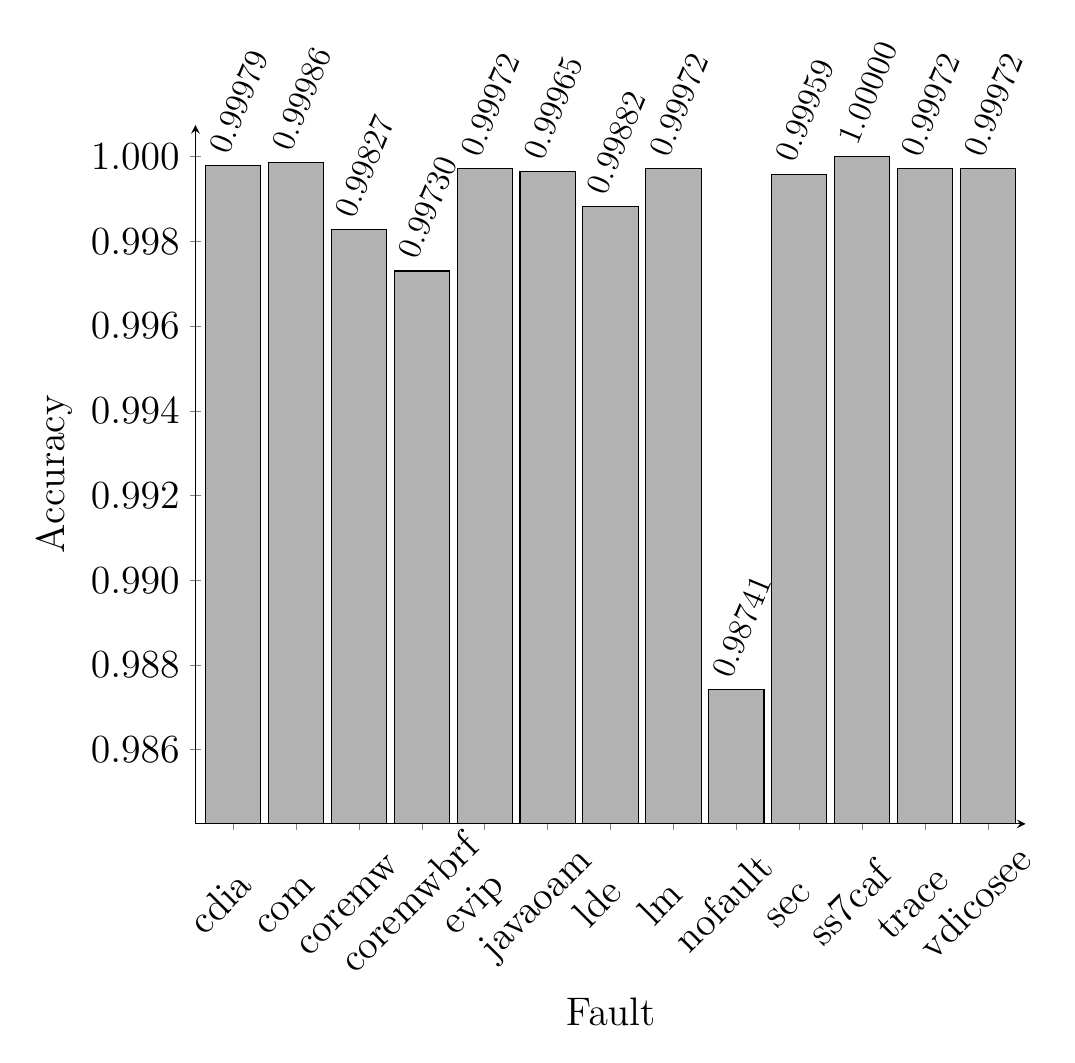
\begin{tikzpicture}[font=\Large]
    \begin{axis}[
      width=\textwidth,
      ybar,
      font=\Large,
      bar width=20pt,
      xlabel={Fault},
      ylabel={Accuracy},
      xticklabel style={rotate=45,anchor=base,yshift=-20,xshift=-22},
      xtick=data,
      ymin=0.985000,
      ymax=1.000000,
      axis x line=bottom,
      axis y line=left,
      enlarge x limits=0.1,
      enlargelimits=0.05,
      domain=0.98500:1.000000,
              y tick label style={
            /pgf/number format/.cd,
            fixed,
            zerofill,
            precision=3,
            /tikz/.cd,},
      symbolic x coords={cdia,com,coremw,coremwbrf,evip,javaoam,lde,lm,nofault,sec,ss7caf,trace,vdicosee},
      nodes near coords={\pgfmathprintnumber[fixed zerofill, precision=5]{\pgfplotspointmeta}},
      every node near coord/.append style={font=\large, color=black, rotate=67.5, anchor=center, xshift=22, yshift=7}],

    ]
      \addplot[fill=black!30] coordinates {
        (cdia,0.999793) (com,0.999862) 
		(coremw,.998271) (coremwbrf,0.997303) (evip,0.999723) (javaoam, 0.999654) (lde, 0.998824) (lm, 0.999723) (nofault,0.987413) (sec, 0.999585) (ss7caf, 1.0) (trace, 0.999723) (vdicosee,0.999723)
      };
    \end{axis}
  \end{tikzpicture}}
    \caption{Classification accuracy of each fault class with complete system logs presented to the HTM model.}
    \label{fig:acc}
\end{figure}




\subsection{Inference With 10 Per Cent Drop-Out}
With a drop-out rate of ten per cent a severe decline in the classification performance is visualised in the confusion matrix, \autoref{fig:10confmatrix}. In \autoref{fig:recall10}, the ability of the HTM model to correctly classify the classes with few examples decreases to below 50 per cent in almost all cases. But in \autoref{fig:acc10}, the accuracy is still very high for all classes except the \textit{nofault} class. The reason for this is that for classes with a small population, the large number of \textit{True Negatives} saturate the metric. However, for the \textit{nofault} class, a major decrease is evident.



\begin{figure}[H]
    \vspace{-.5cm}
    \centering
    \includegraphics[width=\textwidth]{results/figures/256_32_10pcterror.png}
    \caption{The confusion matrix of the classification made by the HTM model with ten per cent word drop-out in each sequence. The vertical axis represent the actual sequence presented to the HTM model, and the horizontal axis represent the predicted fault class.}
    \label{fig:10confmatrix}
\end{figure}
\raggedbottom

\begin{figure}[H]
  \centering
    \scalebox{.61}{    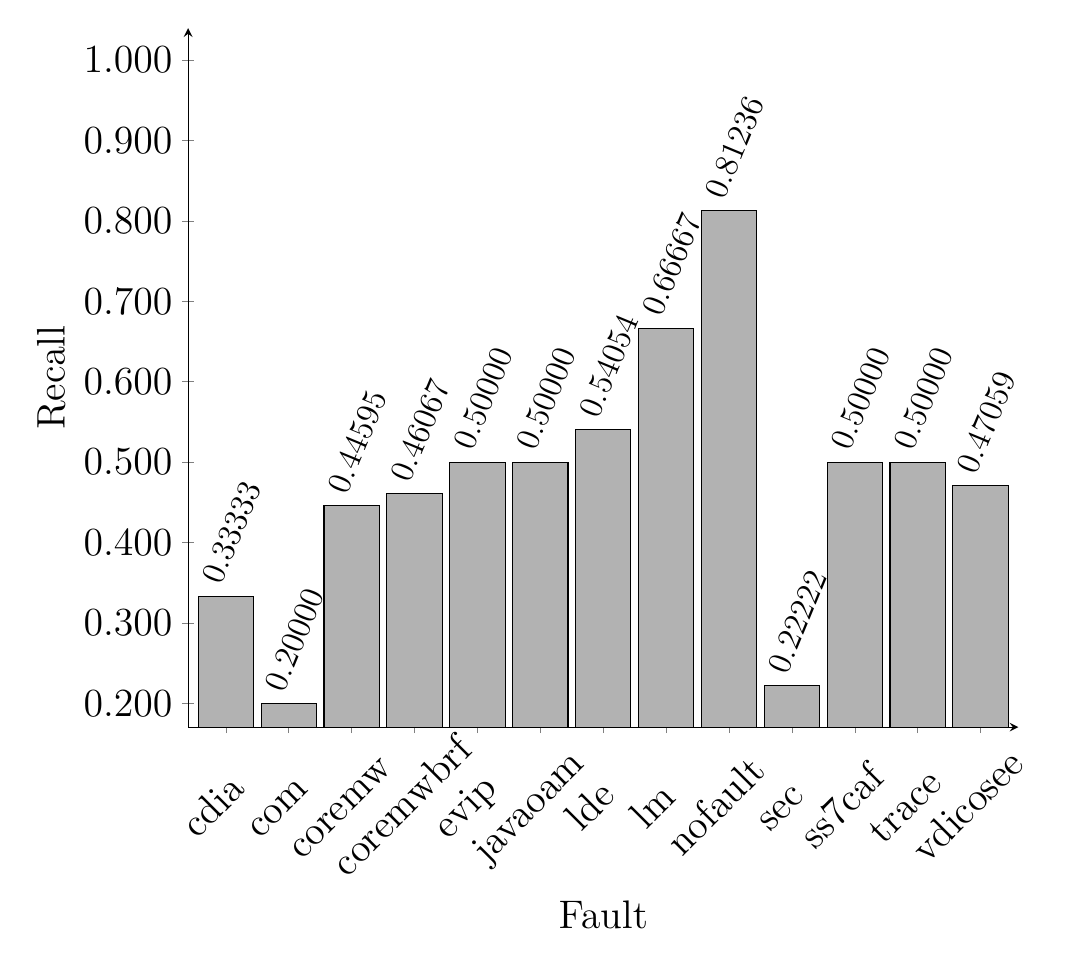
\begin{tikzpicture}[font=\Large]
    \begin{axis}[
      width=\textwidth,
      ybar,
      font=\Large,
      bar width=20pt,
      xlabel={Fault},
      ylabel={Recall},
      xticklabel style={rotate=45,anchor=base,yshift=-20,xshift=-22},
      xtick=data,
      ymin=0.2100,
      ymax=1.00,
      axis x line=bottom,
      axis y line=left,
      enlarge x limits=0.1,
      enlargelimits=0.05,
      domain=0.21:1.000,
              y tick label style={
            /pgf/number format/.cd,
            fixed,
            zerofill,
            precision=3,
            /tikz/.cd,},
      symbolic x coords={cdia,com,coremw,coremwbrf,evip,javaoam,lde,lm,nofault,sec,ss7caf,trace,vdicosee},
      nodes near coords={\pgfmathprintnumber[fixed zerofill, precision=5]{\pgfplotspointmeta}},
      every node near coord/.append style={color=black, rotate=67.5, anchor=center, font=\large, xshift=22, yshift=7}],

    ]
      \addplot[fill=black!30] coordinates {
        (cdia,0.33333) (com,0.2) 
		(coremw,.445946) (coremwbrf,0.460674) (evip,0.5) (javaoam, 0.5) (lde, 0.540541) (lm, 0.666667) (nofault,0.812364) (sec, 0.222222) (ss7caf, .5) (trace, 0.5) (vdicosee,0.470588)
      };
    \end{axis}
  \end{tikzpicture}}
    \caption{Recall of each fault class, with ten per cent word drop-out of each sequence.}
    \label{fig:recall10}

    \vspace*{\floatsep}

    \scalebox{.61}{    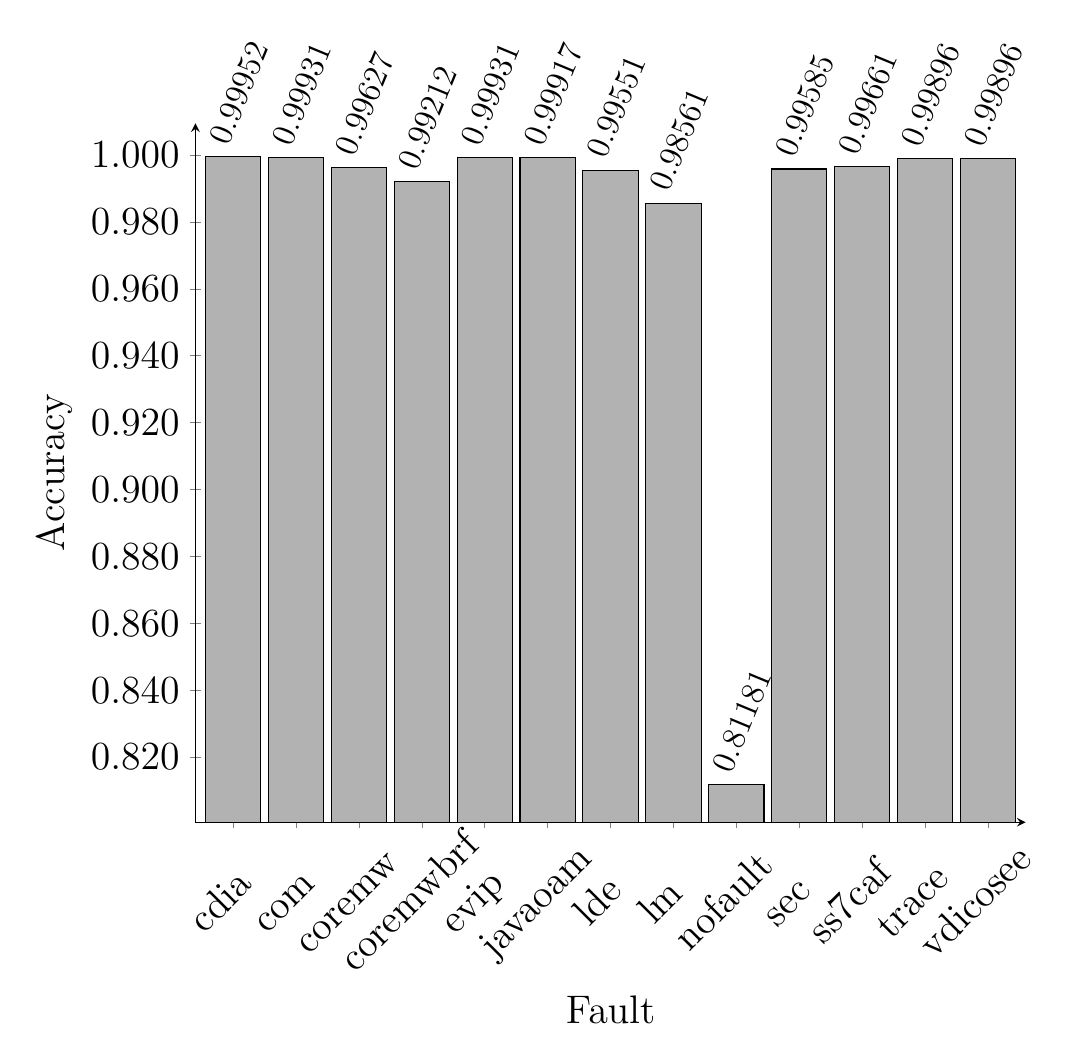
\begin{tikzpicture}[font=\Large]
    \begin{axis}[
      width=\textwidth,
      ybar,
      font=\Large,
      bar width=20pt,
      xlabel={Fault},
      ylabel={Accuracy},
      xticklabel style={rotate=45,anchor=base,yshift=-20,xshift=-22},
      xtick=data,
      ymin=0.81000,
      ymax=1.000000,
      axis x line=bottom,
      axis y line=left,
      enlarge x limits=0.1,
      enlargelimits=0.05,
      domain=0.800:1.000000,
              y tick label style={
            /pgf/number format/.cd,
            fixed,
            zerofill,
            precision=3,
            /tikz/.cd,},
      symbolic x coords={cdia,com,coremw,coremwbrf,evip,javaoam,lde,lm,nofault,sec,ss7caf,trace,vdicosee},
      nodes near coords={\pgfmathprintnumber[fixed zerofill, precision=5]{\pgfplotspointmeta}},
      every node near coord/.append style={color=black, rotate=67.5, anchor=center, font=\large, xshift=22, yshift=7}],

    ]
      \addplot[fill=black!30] coordinates {
        (cdia,0.999516) (com,0.999308) 
		(coremw,.996265) (coremwbrf,0.992116) (evip,0.999308) (javaoam, 0.99917) (lde, 0.995505) (lm, 0.985614) (nofault,0.811813) (sec, 0.99585) (ss7caf, .996611) (trace, 0.998963) (vdicosee,0.998963)
      };
    \end{axis}
  \end{tikzpicture}}
    \caption{Classification accuracy of each fault class, with ten per cent word drop-out of each sequence.}
    \label{fig:acc10}
\end{figure}



\subsection{Inference With 20 Per Cent Drop-Out}
The trend from the previous experiment is continuing with a drop-out of twenty per cent. The pattern in the confusion matrix, \autoref{fig:20confmatrix}, is starting to appear random, which means the HTM model has trouble labelling any class correctly in the majority of cases. However, the fault class \textit{ss7caf} is correctly classified in all cases, but from \autoref{table:dataset} we can see that \textit{ss7caf} only contain two examples. Thus, no real conclusions can be drawn from this, especially since \autoref{fig:recall10} shows that it misclassified \textit{ss7caf} 50 per cent of the time. The severity of the decline is also evident in \autoref{fig:recall20}, with HTM model having a recall of around 20-30 per cent. In \autoref{fig:acc20}, the accuracy is still saturated for all classes except \textit{nofault}, which has now dropped to $59.167$ per cent. 

\begin{figure}[H]
%    \vspace{-.2cm}
    \centering
    \includegraphics[width=\textwidth]{results/figures/256_32_20pcterror_v2.png}
    \vspace{-1cm}
    \caption{The confusion matrix of the classification with twenty per cent word drop-out. The vertical axis represent the actual sequence label presented, and the horizontal axis represent the predicted fault label.}
    \label{fig:20confmatrix}
\end{figure}

\raggedbottom



\begin{figure}[H]
  \centering
    \scalebox{.61}{    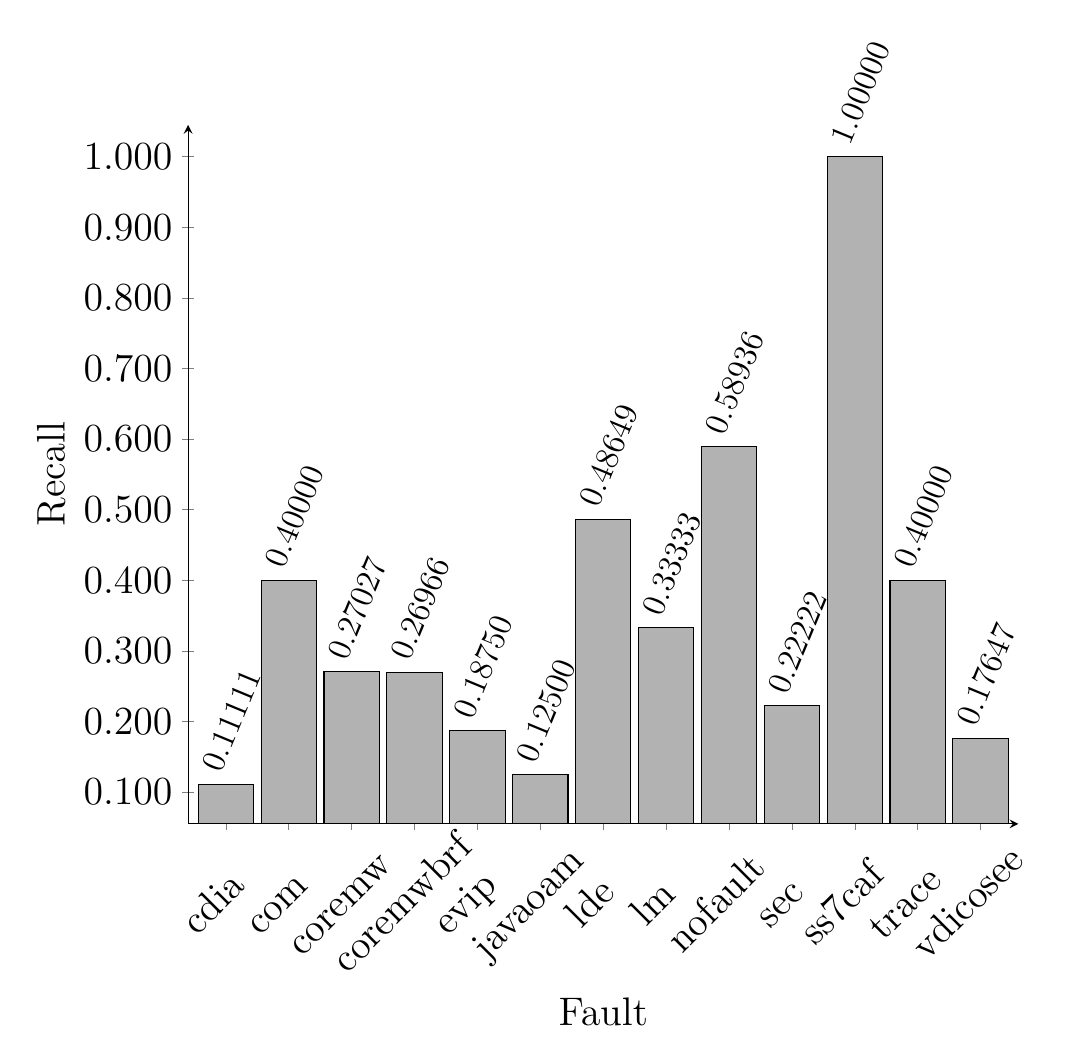
\begin{tikzpicture}[font=\Large]
    \begin{axis}[
      width=\textwidth,
      ybar,
      font=\Large,
      bar width=20pt,
      xlabel={Fault},
      ylabel={Recall},
      xticklabel style={rotate=45,anchor=base,yshift=-20,xshift=-22},
      xtick=data,
      ymin=0.100,
      ymax=1.00,
      axis x line=bottom,
      axis y line=left,
      enlarge x limits=0.1,
      enlargelimits=0.05,
      domain=0.10:1.000,
              y tick label style={
            /pgf/number format/.cd,
            fixed,
            zerofill,
            precision=3,
            /tikz/.cd,},
      symbolic x coords={cdia,com,coremw,coremwbrf,evip,javaoam,lde,lm,nofault,sec,ss7caf,trace,vdicosee},
      nodes near coords={\pgfmathprintnumber[fixed zerofill, precision=5]{\pgfplotspointmeta}},
      every node near coord/.append style={color=black, rotate=67.5, anchor=center, font=\large,  xshift=22, yshift=7}],

    ]
      \addplot[fill=black!30] coordinates {
        (cdia,0.11111) (com,0.4) 
		(coremw,.27027) (coremwbrf,0.269663) (evip,0.1875) (javaoam, 0.125) (lde, 0.486486) (lm, 0.333333) (nofault,0.589362) (sec, 0.222222) (ss7caf, 1.0) (trace, 0.4) (vdicosee,0.176471)
      };
    \end{axis}
  \end{tikzpicture}}
    \caption{Recall of each fault class, with twenty per cent word drop-out of each sequence.}
    \label{fig:recall20}

    \vspace*{\floatsep}

    \scalebox{.61}{    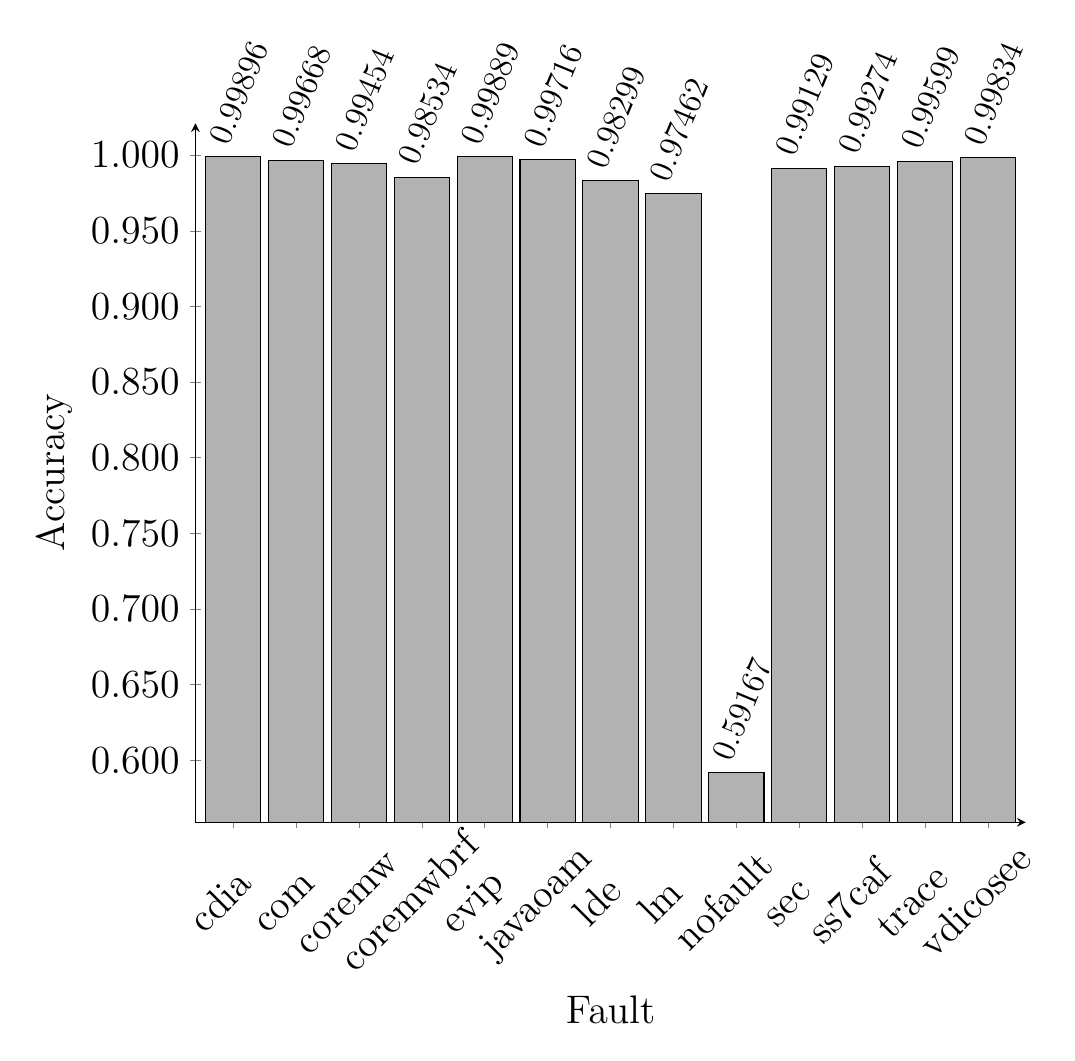
\begin{tikzpicture}[font=\Large]
    \begin{axis}[
      width=\textwidth,
      ybar,
      font=\Large,
      bar width=20pt,
      xlabel={Fault},
      ylabel={Accuracy},
      xticklabel style={rotate=45,anchor=base,yshift=-20,xshift=-22},
      xtick=data,
      ymin=0.58000,
      ymax=1.000000,
      axis x line=bottom,
      axis y line=left,
      enlarge x limits=0.1,
      enlargelimits=0.05,
      domain=0.5800:1.000000,
              y tick label style={
            /pgf/number format/.cd,
            fixed,
            zerofill,
            precision=3,
            /tikz/.cd,},
      symbolic x coords={cdia,com,coremw,coremwbrf,evip,javaoam,lde,lm,nofault,sec,ss7caf,trace,vdicosee},
      nodes near coords={\pgfmathprintnumber[fixed zerofill, precision=5]{\pgfplotspointmeta}},
      every node near coord/.append style={color=black, rotate=67.5, anchor=center, font=\large, xshift=22, yshift=7}],

    ]
      \addplot[fill=black!30] coordinates {
        (cdia,0.998963) (com,0.99668) 
		(coremw,.994536) (coremwbrf,0.985338) (evip,0.998893) (javaoam, 0.997164) (lde, 0.982986) (lm, 0.974618) (nofault,0.591673) (sec, 0.991286) (ss7caf, .992738) (trace, 0.995989) (vdicosee,0.99834)
      };
    \end{axis}
  \end{tikzpicture}}
    \caption{Classification accuracy of each fault class, with twenty per cent word drop-out of each sequence.}
    \label{fig:acc20}
\end{figure}



\subsection{Comparison With Linnaeus}
The final evaluation is a comparison with the already existing classifier \textit{Linnaeus}. If the HTM model should be an viable option in a production setting, it should have comparable or better statistics than \textit{Linnaeus}. However, the machine learning models where benchmarked on different computers, thus contributing to the differences in the timing reports.

The \textit{Linnaeus} model was benchmarked on a computer with an Intel(R) Xenon(R) CPU ES-2658 v2 processor with 40 cores, Skylake microarchitecture, and 2.4 GHz clock frequency. During training 20 cores are utilised at 100 per cent. The HTM model was benchmarked on a computer with an Intel i5-6300U processor with two cores, and with clock frequency of 2.4 GHz. During training and testing of the HTM model one core was utilised at 100 per cent.


In \autoref{tab:stats}, the comparable statistics are presented. We start by introducing the statistics for the \textit{Linnaeus} model. The first two model types are \textit{word n-grams}, where $n$ contiguous words in each system log are bagged together to form a vocabulary. The next two models are \textit{character n-grams}, and instead of words, $n$ contiguous characters are bagged together. Vocabulary build time represents the time it takes to build the different vocabularies based on the model chosen. The total training time is therefore sum of vocabulary build time and training time. The service side is the occupied memory usage when classifying new system logs. The classification latency represents the time it takes to classify a part of a system log file at a time, currently 88 kB at a time. The test accuracy is based on unseen portion of the data set, i.e. the training and testing set were separated. As shown in \autoref{tab:stats}, the accuracy for the models is obtain through several runs where training and testing are split different each time. The accuracy range from $70-95$ per cent for the different models using the test set, and $98-100$ per cent during training.



\begin{table}[H]
\centering
\renewcommand\arraystretch{1.2}
\tiny

\caption{The comparable statistics between the two machine learning models.}
\label{tab:stats}

\begin{tabularx}{\textwidth}{@{} ccccccc}
    \toprule
    &&& &&&\\
    &&\multicolumn{3}{c}{\centering\parbox{5cm}{\centering\large\textbf{Linnaeus Model}}} \\
    &&& &&&\\
    \multirow{2}{*}{\centering\parbox{1.5cm}{\centering \\Configuration}} & \multirow{2}{*}{\centering\parbox{1cm}{\centering Train\\Accuracy}}  & \multirow{2}{*}{\centering\parbox{1cm}{\centering Test\\Accuracy}} & \multirow{2}{*}{\centering\parbox{1.5cm}{\centering Vocabulary\\Build Time}} & \multirow{2}{*}{\centering\parbox{1cm}{\centering Training\\Time}} & \multirow{2}{*}{\centering\parbox{1cm}{\centering Service\\Size}} & \multirow{2}{*}{\centering\parbox{1.5cm}{\centering Classification\\Latency}}\\
    &&&&&&\\
    \midrule
            Word ngrams = 1 & $99\%$ & $75-95\%$ & 42 s &150 s& 150 MiB & 10 ms\\
            Word ngrams = 2 & $98\%$ & $75-95\%$ & 109 s &217 s & 150 MiB & 17 ms\\
            Char ngrams = 2 & $100\%$ & $70-95\%$ & 787 s &787 s & 150 MiB & 68 ms\\
            Char ngrams = 4 & $99\%$ & $70-95\%$ & 514 s &514 s& 150 MiB & 42 ms\\
    \bottomrule
\end{tabularx}


\begin{tabularx}{\textwidth}{@{} ccccccc}
    &&& &&&\\
    \multicolumn{6}{c}{\centering\parbox{5cm}{\centering\large\textbf{HTM Model}}} \\
    &&& &&&\\
    \multirow{2}{*}{\centering\parbox{2cm}{\centering \\Experiment}}    & \multirow{2}{*}{\centering\parbox{2cm}{\centering Train\\Accuracy}}   &\multirow{2}{*}{\centering\parbox{1.5cm}{\centering Build\\Time}} &\multirow{2}{*}{\centering\parbox{2cm}{\centering Training\\Time}} & \multirow{2}{*}{\centering\parbox{1cm}{\centering Service\\Size}}&\multirow{2}{*}{\centering\parbox{2cm}{\centering Classification\\Latency}}&\\
    &&& &&&\\
    \midrule
    $0\%$ drop-out & $98.6\%$      &131 s      &828 s        &888 MiB     &88 ms&\\
    $10\%$ drop-out& $80.7\%$     &--        &--         &888 MiB     &88 ms&\\
    $20\%$ drop-out& $58.5\%$      &--        &--          &888 MiB     &88 ms&\\
    \bottomrule
\end{tabularx}
\end{table}


Let us now introduce the statistics of the HTM model, also presented in \autoref{tab:stats}. Instead of model configurations, we present the accuracy obtained from the model during the three experiments performed. We can see a clear degradation of the accuracy as we introduce faults into the system log sequences, from 98.6 to 58.5 per cent. The reason we preformed this test is to see how well the HTM model preformed with added errors to the sequences. This test is however not really comparable to the \textit{Linnaeus} models, but it does tell us how well it is at classifying incomplete system logs. Next, we have the build time, which is the time it takes to perform all the preprocessing steps required. The training time represent the time it took to train the HTM model using \textit{one-shot learning}. Service size is the memory usage of the HTM model. An important thing to note is that the most of the memory usage is due to the allocation lists used for encoding, decoding, and the entire system log data set. The network size is only 178 MiB of the entire 888 MiB. Classification latency is the time it takes to encode each word to an SDR, present it to the HTM model, and decode a prediction at the end of a system log sequence. 


From comparing the statistics, the \textit{Linnaeus} models achieves similar results in the training cases as the HTM model. The classification of the system logs are performed in different ways, where the \textit{Linnaeus} model takes system log chunks and processes them, where as the HTM model looks at individual logs, one at a time. It is likely that the execution time for all parts of the HTM model would be faster if it where evaluated on a better machine. But with current metrics, the \textit{Linnaeus} model has the benefit have lower classification latency and smaller memory footprint, i.e. service size.

The test with 10 and 20 per cent dropout with HTM model is interesting, as they give some indication on how well the model is at being able to classifying system logs if the vocabulary is changed. However, with the current HTM model we can see that it does not adapt well to introduced errors in the system log sequences. 



%176MB Network size
%DISCUSSION AND CONCLUSION
\chapter{Discussion and Conclusion}
\label{chp_disc}
In this chapter we discuss and summarise the results obtained and presented in the previous chapter. We start off with explaining why we used the entire dataset for training and testing. Then, we discuss the results and the evaluation. Next, we discuss the model and the design choices made. Finally, we give a conclusion of this work, future improvements, and ethics. 


\section{Discussion}
The main objective of this thesis was to create and compare an \textit{Hierarchical Temporal Memory} (HTM) model with the existing system called \textit{Linnaeus}, in order to evaluate if the HTM algorithm is a suitable choice for anomaly detection of system logs. First, we discuss the results presented in \autoref{chp_res}. Then we will go over the choice of method where we discuss the data and the HTM model. An important note to make before we start the evaluation, is to state that the HTM model was trained and tested on the entire data set. The choice for this will be discussed further under the \textit{Data} subsection.  

\subsection{Data}
The data set contained a set of examples of system logs classified by a technician to be the reason for causing a specific fault. During the thesis there was no possibility of expanding this data set with more examples. To manually go through unlabelled data sets would require domain expertise. 

Due to the fact that the HTM model was evaluated on the data set that it was trained on. It is important to state the reason why before we start discussing the performance of the algorithm. The decision not to split the data set into a training and testing set was made for the following reasons:

\begin{itemize}
    
    \item The data set was heavily skewed, where 95.2\% of 14459 labeled examples belonged to the \textit{NoFault} class.
    
    \item For some of the classes with few examples, there was no underlying pattern, meaning that they did not use the same vocabulary. Therefore, no machine learning algorithm would be able to correctly classify the other system log while only being trained on the first example. 
    
\end{itemize}


\subsection{Results}
The results gathered to evaluated the HTM model are based on three metrics describe in \autoref{sec:metrics}. First, we used the \textit{Confusion Matrix} to visualise the performance of the classifications. Then, we presented the \textit{Recall} and \textit{Accuracy} for each experiment.


During the first experiment we did not alter the system logs in any way. The performance of the HTM model is rather impressive even though it is tested on the training set. The reason that the results show promise is that the model was trained using \textit{one-shot learning}. But it is also impressive due to the distribution of the dataset, where there is a possibility that any machine learning model would over-fit on the \textit{NoFault} class. 

It would however been interesting to evaluate the system using \textit{multi-shot learning}. But as the entire dataset was used for training and testing, the risk of over-fitting would have been great. If the distribution of the samples in the dataset was different, \textit{multi-shot learning} would have been an interesting choice, where the model would be evaluated on unseen examples.


However, with \textit{one-shot learning} the HTM model it is less likely to over fit on during training. Therefore, some conclusions can be drawn from the results gathered. As we see in \autoref{fig:confmatrix}, the diagonal is prominent for the first experiment, meaning that the model is able to make correct predictions most of the time. If we then move on to study the recall and accuracy figures, shown in \autoref{fig:recall} and \autoref{fig:acc} respectively, we see that the model had an overall satisfactory performance, meaning that it had over $70\%$ recall on most classes. The accuracy throughout all experiments does not tell us a whole lot about the performance of the model. The reason for this is that this metric is saturated by the sheer size of \textit{True Negatives} for all classes except the \textit{NoFault} class.


The trend of decay in performance is present in both of the following experiments when errors in the sequences are introduced. Which is a likely scenario if new words are introduced by a developer. A reason for this poor performance has to due with how the HTM algorithm learns sequences. Much like the a human with reading comprehension can recite the alphabet forward, every thing is done in sequence of sequences, e.g. \textit{''abcd''} then \textit{''efg''}. But if a human asked to change something in this learnt sequence before reciting it, e.g. reciting the alphabet backwards, he will find it impossible to do, unless he knows it beforehand. This is because the brain and the HTM algorithm learns forward sequence of sequences \cite{Kurzweil:2013:CMS:2534455, 10.3389/fncir.2016.00023}. When a sequence with drop-out is presented to the HTM algorithm, the columns will be \textit{bursting} due to the unpredicted input pattern, which will have consequences on future predictions.  


\subsubsection{Evaluation}
The evaluation is not obvious to make based on the acquired results. This is mainly due to the fact that the accuracy is not a good metric on a data set with an uneven distribution between the classes. This is due the fact that the size of the \textit{True Negative} population will saturate the accuracy for the classes with few examples. To quantify the performance of the two models, access to real test logs files would almost be necessary. But to do a fair comparison between the models with the statistics presented in \autoref{tab:stats}, we should use the training accuracy of the \textit{Linnaeus} model. We can then see that they are almost identical in performance. However, the results from the \textit{Linnaeus} model could be over-fitted, due to the fact that most no noise or errors, e.g. drop-out, where introduced during training or testing. The advantage of HTM model is that it used \textit{one-shot learning}, thus minimising the risk of over-fitting. However, HTM model does not optimise over a parameter space either, as it uses a Hebbian style learning, which should make it less prone to over-fitting the data in any case. 

In terms of classification speed, \textit{Linnaeus} is between 11 and 48 per cent faster. The computational time could largely be due to the fact that they where trained and tested on two different computers, \textit{Linnaeus} on a powerful desktop and the HTM model on a laptop. However, the NuPiC framework that the HTM model uses for the temporal memory algorithm does not support multi-core processing. So the speed-up would be somewhat limited. With this said, the HTM model could be optimised by looking over parts of the code that is inefficient, e.g. the encoding and decoding function. 

An obvious benefit of using a system log classifier based on the HTM algorithm is that when new system logs are introduced, retraining on the whole system log database is not needed. It would be enough to only present the new system logs to the HTM model. This is because the HTM model does not optimise weights given a certain input, as in traditional machine learning techniques. Instead, input patterns are learned via the change of permanence values in the synaptic connections of each HTM neuron. Thus, making the model robust to changes in the system logs.


\subsection{Method}
In this subsection we will discuss the design choices made in the implementation of the model. 

\subsubsection{Model}
There are two parts in the implementation that could be analysed; the encoding of words into Sparse Distributed Representations (SDRs), and secondly the network architecture. 

The performance of the HTM model is heavily dependent on how well information is encoded into a Sparse Distributed Representations (SDRs). A drawback to our implementation is that it is hard to evaluate the GloVe encodings, as the word vector space is created by a corpus of all system logs. The system logs themselves, as shown in \autoref{fig:prosyslog}, are not structured messages in the sense that analogies that be derived from them. This could in turn mean that the GloVe encodings are sub optimal when encoding words into SDRs. This could mean that dissimilar words or acronyms are encoded as SDRs that share on bits, which could then confuse the temporal memory to confuse system log sequences. 


Lastly, the HTM model is a one layer temporal memory with 32 cells in each of the 256 columns. The reason for limiting the network to one layer was that predictions of future inputs from this layer could be easily extracted and decoded. Reports, such as \cite{7844355}, indicates that one layered temporal memory is enough to create a state-of-the-art text generation algorithm. With more layers the size of the service size of the model would have increased, which was not inline with goal of this thesis.






\section{Conclusion}
The HTM model has shown promise in classification of system logs. It preforms well with limited computational resources and is able to classify system logs rather well with \textit{one-shot learning}. The author believes that a claim regarding the use of an HTM model in a production setting would be easier if a more thorough benchmark was made, e.g. system log files from real test was presented to both classifiers, and then compare metrics. But with the current knowledge, the author believes that an HTM model for this task would be preferable due to the fact that the model does not need to be retrained on the entire data set when new examples are introduced. 






\section{Future Work}
The first major improvement to be made would be to train the HTM model on system log sequences with different drop-out rates to see if the HTM model is able to learn to generalise. 


The drop-out experiments tries to recreate the situation when a new word is introduced and the encoder is not able to encode it into an existing SDR. However, instead of just passing on to the next word in the sequence, it would be interesting to pass the prediction from the previous time step in as the input SDR to the network. This would prevent some columns from bursting, where all cells become active, and minimise this impact on the future prediction and the prediction of the fault class.


The next improvement could be to change the structure of the HTM model and remove the temporal aspect of viewing the system logs, and instead use an approach similar to \textit{coritcal.io} \cite{DBLP:journals/corr/Webber15} with a semantic fingerprinting (SDR) of each system log. The semantic fingerprints would be created by, as before, first creating a unique SDR for each word. By aggregating all the SDRs of a sequence together, each index would increment for each ON bit in each SDR. To preserve the spareness of the new SDR, a threshold would be introduced to only convert the indices with the largest accumulated values into a new sparse SDR, while the indices below the threshold would be converted to OFF bits. These semantic fingerprints would then be presented to a spatial pooler, which is a temporal memory without the temporal aspect taken into account. The advantage of this approach would be that the noise tolerance of the HTM theory could be used to its fullest potential, as noise of up till 50 per cent in an input SDR can be handled by an spatial pooler or temporal memory \cite{10.3389/fncir.2016.00023}. 


Another interesting approach would be to find patterns of conditional probabilities between logged events, in order to find faults in system log files. This task could be suitable for an HTM algorithm due to the sequential nature of this task.


A final interesting improvement would be to translate all the Ericsson acronyms into English words. This would then mean that a GloVe model would not be needed to be retrained when new ones appear. We might then be able to use a pretrained GloVe model on the first 6 billion tokes on English Wikipedia.  




\section{Ethics}
The ethical aspects of this thesis and the proposed implementation does not in its current form present much of an ethical issue. This is largely because this model is contained to only analyse system logs gathered in testing. Therefore, the impact of its use is limited, as it will not impact a product providing a service to Ericsson's customers. The intent of this system is not to replace anyone, as this will only be a tool in which a technician could rely on when doing troubleshoots and classifying system log files correctly. And if the system did not perform well enough to reliably help a technician, the system would not be used. 


The ethical aspect could instead be discussed on the topic of machine learning at large. Where there are numerous ethical issues that could arise when implementing machine learning software. From use in autonomous cars to weapon systems. But as these subjects are not part of this thesis we will not dwell further into these never ending philosophical debates. 


\newpage
\printbibliography

\newpage
\appendix
\chapter{The Neuroscience of the Neocortex}
\label{chp_neocortex}
This is a complementary chapter to \textit{''A Brain-Inspired Algorithm''}. We will go through some of the neuroscience of the \textit{new cerebral cortex} (neocortex), that the \textit{Hierarchical Temporal Memory} (HTM) theory is biologically derived from. We being by introducing the neocortex of the mammalian brain and why it is believed to be the part of the brain where intelligence resides. Then, the topology of the neocortex is presented, where we will go through the structure of each layer. Next, we describe the columnar organisation of the neocortex, first coined by Vernon B. Mountcastle, which is one of the main inspirations in HTM theory. We then continue to describe the neural circuitry of these cortical columns. Finally, we introduce the pyramidal neuron, which is the most frequently occurring type of neuron that resides in the neocortex. The HTM neuron is modelled on the pyramidal neuron's functionality and the active processing properties of its dendrites. 


\section{The Neocortex}
What separates all mammals from the rest of the animal kingdom is the existence of the neocortex in the cerebral cortex \cite{Neocortex}. The neocortex is perceived as the part of the brain where intelligence resides. The reason for this is that the neocortex is responsible for higher order brain functions, such as sensory perception, advanced motor control, association, memory, and cognition \cite{LodatoSimona2015GNDi}.  



\begin{figure}[ht!]
    \centering
    \begin{tikzpicture}
        \node[anchor=south west,inner sep=0] (image) at (0,0)
        {\includegraphics[scale=.35]{appendix/neuroscience/figures/brain2.png}};
        \node [anchor=west] (Neocortex) at (1,7) {Neocortex};
        \node [anchor=west] (Old Brain) at (3,1) {Old Brain};
            \begin{scope}[x={(image.south east)},y={(image.north west)}]
                \draw [-latex, thick, black] (Neocortex) to[out=0, in=120] (0.45,0.91);
                \draw [-latex, thick, black] (Old Brain) to[out=0, in=-120] (0.6,0.1);
            \end{scope}
    \end{tikzpicture}%
    \caption{\cite{BrainSketch} A sketch of the brain of a Homo sapiens. The cerebral hemisphere is recognised by the convoluted form with ridges and furrows.}
    \label{fig:forebrain}
\end{figure}


The forebrain, shown in figure \autoref{fig:forebrain}, is the largest part of the mammalian brain, made up of the cerebrum, thalamus, and hypothalamus. The cerebrum is made up of two cerebral hemispheres. The cerebral hemisphere has an outer layer of grey matter and the cerebral cortex beneath it \cite{crossman2014neuroanatomy}. The cerebral cortex consists of two areas, the neocortex and the allocortex, defined by their cytoarchitecture \cite{Allocortex}. The neocortex is larger in area and it is the outer most layer of the cerebral cortex, organised into six horizontal laminae of neurons. The allocortex is smaller in size with subareas such as the hippocampus, subiculum and olfactory cortex \cite{Neocortex}. Because mammals share the same brain structure of the olfactory cortex and the hippocampus with reptiles but not the neocortex, it was long viewed that the neocortex was a new evolutionary addition of the brain, hence the name. However, the neocortex should instead be viewed as homologous with the dorsal cortex of reptiles. Though, the difference between them is noticeable, the neocortex is a thick, laminated and uniform structure containing abundance of neurons; compared to the dorsal cortex in reptiles which contains only about a row of neurons in its sheet of tissue \cite{Neocortex}. With these dissimilarities in mind, the function of all vertebrate brains is still the same, which is to act as a premotor organ that sends motor commands to the animals' muscles \cite{10.3389/fnana.2013.00051}. 


What makes the human neocortex so special that its able to give us humans the ability to express our thoughts through motor commands, e.g. writing or speaking, perception, imagination, language processing and cognition? One major factor to why humans surpasses it counterparts in intelligence is the sheer size of the neocortex, a surface area of roughly 2600 cm$^2$ and a thickness of 3-4 mm, together with the vast number of neurons, up to $28\times10^9$, that resides there \cite{MountcastleVernon1997}. The human neocortex wraps around the forebrain in a convoluted fashion, compared to a rodents' neocortex which is non-folded. This allows the human neocortex to have more surface area with a limited volume \cite{folded}. Another reason why humans surpasses all other mammals is evolutionary, i.e. having a large neocortex with many subdivisions is metabolically costly, takes a long time to develop and mature and is unnecessary for most other animals \cite{Neocortex}. 


\subsection{The Topology}
The neocortex organized in hierarchy of six horizontal stacked laminae, numbered I--VI, with each of the layers grouped based on synaptical connectivity, morphological type of neurons and at which depth they exist \cite{Neocortex}. This basic structure is shown in \autoref{fig:layers}. To understand the difference of each layers' topology and processing properties, a brief description is given below:



\begin{itemize}[leftmargin=4em,align=left]
    \item \textbf{Layer I:} The top layer, which is mostly inhabited by fibers that run parallel to the surface. The fibers consist of the ends of apical dendrites and axons that connect to each other via synapses, together with a few neurons. This layer serves two purposes; first, to work as a feedback connection from other cortical areas. Secondly, to modulate input from the brain stem \cite{Neocortex}.
    
    \item\textbf{Layer II:} This layer has a large population of small neurons. The dendrites of these neurons are connected to neighbouring cortical areas and pyramidal neurons in deeper layers via their apical dendrites. Thus, allowing intracortical connections to affect the processing in a local area \cite{Neocortex}.
    
    \item\textbf{Layer III:} One of the main output layers of the neocortex, consisting of medium sized pyramidal neurons with basal and apical dendrites. The axons of these neurons serves as commissural fibers, i.e. connections between the two cortical hemispheres, and as connections to other cortical areas \cite{crossman2014neuroanatomy}. The pyramidal neurons receive their input form other layers in the local area via their apical dendrites. Adjacent neurons in layer III are able exchange information via their basal dendrites. This layer is of great importance, as it makes it possible for information exchange between regions in the neocortex. Thus increasing the complexity of possible operations that can be performed \cite{Neocortex}.
    
    \item\textbf{Layer IV:} The main input layer and situated in the middle occupied by small stellate cells. The name is given due to the radial propagation of the dendrites. The information that the stellate cells receives is shared locally between neighbours via the basal dendrites and then transmitted to the adjoining layers above and below. The stellate cells are small due to the fact that the axons and dendrites only extend a short range \cite{Neocortex}.
    
    
    \item\textbf{Layer V:} This is the other main output layer of the neocortex. Large pyramidal neurons inhabit this layer, which can be seen in \autoref{fig:layers} as triangular black spots. The main task of this layer is to integrate information from both its horizontal neighbours and all vertically connected neurons in the layers above up till layer I that belongs to the same cortical column \cite{Neocortex}. This information is then sent out to extra-cortical parts of the brain, i.e. basal ganglia, thalamus, brain stem and the spinal cord, via long axons \cite{crossman2014neuroanatomy}. But also to remote cortical areas, including areas in the other cerebral hemisphere. As these distances can be quite far and information needs to travel fast, the axons needs thick, as this allows for faster conduction rates. To gather information from the vertically adjoining layers, the apical dendrites branch out in long vertical fibers, with synaptic connections in each layer. Neighbouring cells communicate via their basal dendrites. For the pyramidal neurons to be able to send and receive action potentials on their long apical dendrites, and also thick axons the cell body needs to be large \cite{Neocortex}.
    
    
    \item\textbf{Layer VI:} Until this layer, the information has just been processed in a feed-forward manner, i.e. receive information, manipulate it and transmit it onward to other regions. But bi-directional communication is necessary in any complex computational unit, and this is where layer VI comes in. This is the main feedback layer to other activation regions about the state of the local area. The pyramidal neurons that resides in layer VI mainly get their input for layer IV, as well as direct input from axons that terminate in layer IV. With these connections, layer VI is able to project back information to the neurons in another cortical area that contributed to the activation \cite{Neocortex}. 
    
    
\end{itemize}

\begin{figure}[H]
    \centering
    \includegraphics[scale=.88]{appendix/neuroscience/figures/layers.jpg}
    \caption{\cite{IVIlayers} The cross section above, visualises the general structure of the neocortex categorised into six horizontal laminae, I--VI, on the basis of cytoarchitecture. The cell bodies of the neurons are shown as the darkened spots, neither the axons nor dendrites of the neurons are visible. The white matter connects the neocortical region to other regions in the neocortex along with other parts of the brain. These connections allows the region to send and receive signals \cite{Neocortex}.}
    \label{fig:layers}
\end{figure}

\noindent With the understanding of each layers' properties we can now move on to explain the most basic processing unit of the neocortex, the \textit{minicolumn} and the \textit{cortical column}.

%COLUMNAR ORGANISATION
\subsection{Columnar Organisation}
The most basic processing unit in the neocortex is called a \textit{minicolumn}, first described by Vernon B. Mountcastle in 1955--1959 \cite{doi:10.1093/cercor/13.1.2}. A minicolumn is a vertical array of neurons connected to each other like a chain across layer II--VI. These minicolumns have transverse diameter of 50--80 $\mu$m and contain between 80--100 neurons in primates, but can contain up to 2 times more in the striate cortex. The structure of the minicolumn can be observed throughout the neocortex, however they are not identical as some features differ, e.g. cell phenotypes, synaptic transmitters \cite{doi:10.1093/cercor/13.1.2}. A \textit{cortical column} is a group of minicolumns which is formed by a common input and the horizontal links they have with each other. The number of minicolumns that a cortical column contains varies between 50--80 \cite{doi:10.1093/cercor/13.1.2}. The cortical column functions as a complex distributed system, where each minicolumn can be viewed as a computing node, which is able to modulate inputs and use bilateral communication with neighbouring minicolumns and cortical columns. This allows the cortical columns to link multiple inputs to multiple outputs \cite{MountcastleVernon1997}.


\subsection{Neural Circuit Functionality}
In each minicolumn there exists two types of neurons; the \textit{excitatory neurons}, i.e. pyramidal and spiny stellate cells; and the \textit{inhibitory neuron}, the aspiny stellate cells. The neurons are distributed throughout the layers in the minicolumn with the majority, $\sim$80\% , of the neurons being of the excitatory type \cite{Neocortex}. The excitatory neurons are able to depolarise the neurons of which it is synaptically connected to by sending out a excitatory neurotransmitter, glutamate. In this depolarised state the effected neuron is more likely to itself send out an action potential if it receives strong enough signal on its dendrites \cite{Neocortex}. The opposite is true for the inhibitory neuron, as it sends out an inhibitory neurontransmitter, i.e. a biochemical called \textit{gamma-Aminobutyric acid}, or GABA, which hyper-polarises the effected neuron, making it less likely to produce an action potential. This inhibitory effect allows a local circuit to remain sparse, as minicolumns that respond to the same input tend to inhibit each other. This limits the response time for an input and makes the cortical column sensitive to temporal changes \cite{Neocortex}. 


 The cortical columns are able to correlate different inputs based on interconnections that exist in layer III, as these makes horizontal connection in between cortical columns. The advantage of such connections are that neurons in different cortical columns can become active at the same time, thus being able to respond to the signal of the same object and giving it cohesion \cite{Neocortex}. Another crucial part of the neural circuits is its plasticity. The synaptic connections between neurons change over time, either they become stronger or weaker, which makes the brain able to adapt to new input. This is largely due to the two types of membrane receptors that exist, i.e. the \textit{N-methyl-D-aspartate}, or NMDA, receptor and the non-NMDA receptor. The non-NMDA receptor reacts when glutamate is released, which leads to depolarisation of a neuron. When this happens, the NMDA receptor, which is otherwise blocked by magnesium ions, is unblocked and can pass calcium ions through if another glutamate release occurs in a short amount of time. This leads to a fast succession of action potential being generated by the neuron. Because of this, synaptic strength between the the neurons is increased, which is called long-term potentiation. The opposite is called long-term depression, which means that the neurons does not respond to the same input and their synaptic connections are weakened \cite{Neocortex}. This alteration of the synaptic strength between neurons is also known as Hebbian learning \cite{CapaldiE.John1992TOOB}. 
 
 It is in these synaptic connections that memories are stored. Memories are stored in a sequences and can be recalled auto-associatively. This makes the neocortex robust to noise and incomplete input patterns, as it can auto-complete as input patters as memories are recalled in an ordered sequence. Thus, the neocortex is able to make predictions about the future based on incomplete input \cite{memory}. 

\section{Pyramidal Neuron}
\label{sec:dendrite}
The most abundant of all neuron types in the neocortex is the pyramidal neuron. The pyramidal neuron is unique to the cerebral cortex and can be found in all layers except the first and represent between 70-85\% of the total population in any cortical area. It has therefore been seen as the principle neuron of the cerebral cortex \cite{PyramidalPop}. As the name indicates, the cell body, or \textit{soma}, of the pyramidal neuron has a pyramidal shape, which can be seen in \autoref{fig:pyramidal}.


\begin{figure}[ht!]
    \centering
    \includegraphics[scale=.3]{appendix/neuroscience/figures/PyramidalNeuron.png}
    \caption{\cite{PyramidalPop} A sketch of a stereotypical pyramidal neuron, with a apical dendrite branching out from the apex of the soma, the basal dendrites extends out in the horizontal direction and the axon is descending from the soma.}
    \label{fig:pyramidal}
\end{figure}


\subsection{Dendrites, Synapses and Axons}
The \textit{dendrites} are the input branches of a neuron, which is either able to excite or inhibit the neuron based on the neurotransmitter it receives on its \textit{synapses}. The synapses are the connections between the output branches, or \textit{axons}, and the dendrites, that allows electrical or chemical signal to be transmitted. An axon is the main output branch of the neuron, and is able to transport the signal, or action potential, to its synapses. In the dendrites the input signals are integrated, which in turn changes the state of the neuron if a complex set of conditions are met. Firstly, the integrated signal at a spatial position on the dendrite branch needs to exceed a threshold. This threshold is dynamic as the integrated signal needs to be stronger if its further away from the soma. The second condition that needs to be met is the timing of the synaptic conductances that occur at the integration zone \cite{PyramidalNeuron}. The dendrites can be classified into three zones, the \textit{basal}, \textit{proximal} and \textit{distal} zone. The basal zone contains the basal dendrites that extend along the horizontal axis and connect to neighbouring neurons in the cortical column. The apical dendrite can be divided into two parts, a proximal zone, closer to the soma, and the distal zone which is further away. In the distal zone the amplitude of the integrated signal needs to be higher in order to effect the cell state, due to the longer travel distance. The pyramidal neuron is believed to act as a coincidence detector as its been shown to respond best to simultaneous stimulation in distal and proximal areas of the apical dendrite \cite{PyramidalNeuron}. Another important feature of the pyramidal neurons is its ability to adapt to change in the temporal input patterns. It able to change functionality due to synaptic plasticity, which is ability to change the strength of the synaptic connection between neurons \cite{PyramidalNeuron}. As explained in the previous section, the strength of the synaptic connections alters with long-term potentiation or long-term depression.

\section{Summary}
To summaries, HTM theory is derived from properties of the neocortex and the ideas of Vernon B. Mountcastle's single cortical algorithm for information processing. This chapter aimed to familiarise the reader with the structure and functionality of neocortex. First, a gentle introduction to the neocortex was given. Then, we proceeded to the topology and the structure of the individual layers. Next, cortical columns and the neural circuitry was presented, which HTM theory tries to reverse engineer to some extent. Finally, we presented the pyramidal neuron and the functionality of the dendrites. As this is the most abundant neuron in the neocortex, and the inspiration of the HTM neuron's functionality.





%To achieve true machine intelligence one must first be able to understand the information processing that occurs in the brain. Some AI researchers have discarded the idea of this principle with the argument that neither planes nor cars function in the same way as their biological counterparts \cite{Hawkins:2004:INT:993636}. However, intelligence should be defined as the methodology by which an autonomous agent is able to learn in the world \cite{Intelligence}. This means that intelligence resides in the inner workings of the brain and is not equivalent to behaviour. With this definition of intelligence; current state-of-the-art AI agents that can outperform humans in some specific tasks, such as image classification or Go, cannot be seen as intelligent. 



%Geoffrey Hinton, who is hailed as one of the godfathers of Deep Learning is ''deeply suspicious'' of the learning algorithm of Artificial Neural Networks called Back-Propagation, and encourages graduates to scrap this idea and explore new possibilities of learning for neural networks \cite{Hinton}.

%The goal of AI research is to create a Artificial General Intelligence that is on par or surpasses human intelligence. But what makes the human brain so special? It is the size of the \textit{new cerebral cortex} (neocortex) \cite{Neocortex}.
\newpage

\includepdf[fitpaper=true, pages={2}]{FrontAndBackPage/neurobio.pdf}
\end{document}
\endinput
%%
%% End of file `kth-ex1.tex'.
